\chapter{Mechanical Assembly}

\graphicspath{{./Figures/Mechanical Assembly/}}

%\begin{itemize}
%	\item Intro Overview of the chapter.
%	\item Importance of mechanical assembly in the overall project.
In this chapter, the mechanical assembly of the robot is discussed.
The mechanical assembly is the process of putting together the mechanical components of the robot.
The mechanical components include the chassis which is composed of several parts, the wheels, the motors.
The assembly process is described in detail, including the tools and techniques used.
The integration of the mechanical and electronic systems is also discussed.
The challenges faced during the assembly process are described, along with the troubleshooting and problem-solving strategies employed.
Finally, the safety considerations taken during the assembly process are discussed.
, the wheels, the motors.
%\end{itemize}
\newpage

\section{Components Overview}

%\begin{itemize}
%\item Detailed description of all mechanical components used in the robot.
%\item Source or method of fabrication for each component (e.g., machined parts, 3D printed elements).
%\end{itemize}
As shown in the mechanical design chapter, the robot is composed of several mechanical components.The body, hip knee links, knee wheel links, board mounting rack, Wheel motor cover, body cover and body face shield.
These components were printed using a 3D printer with different configuration for each part.Other components such as the wheels, motors, motor shaft hub, screws and thread inserts were bought from the market.
\section{Fabrication}
% figure for printing the body
\begin{figure}[h]
	\centering
	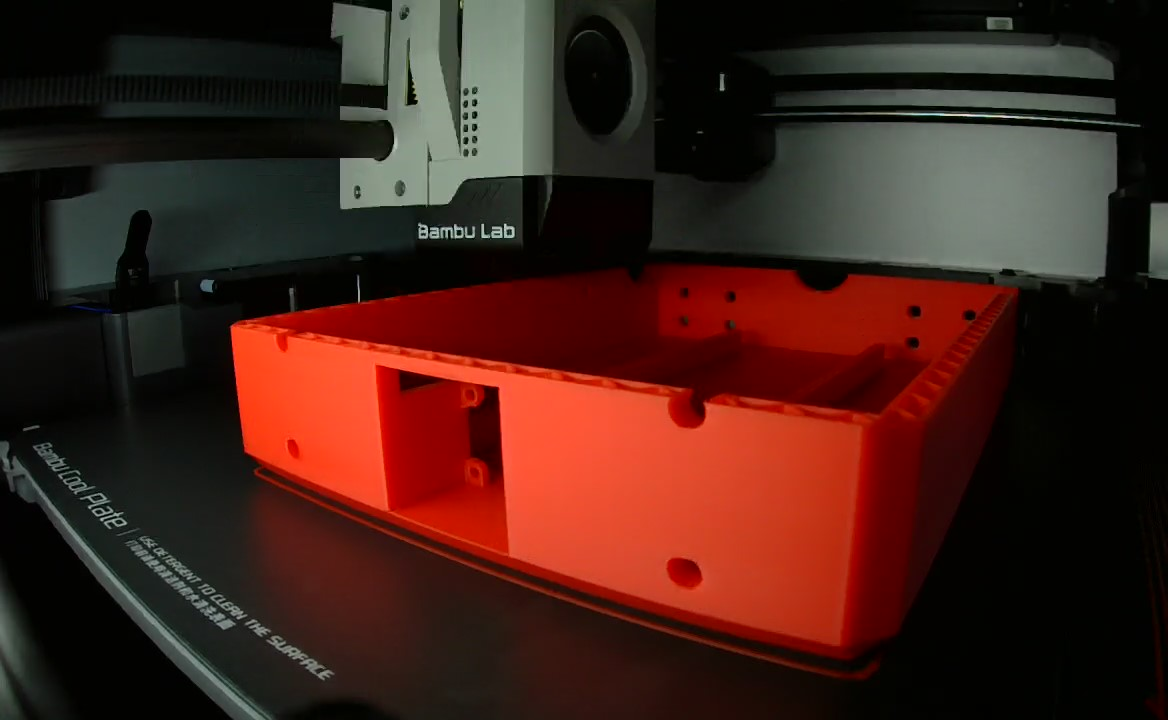
\includegraphics[width=0.7\linewidth]{body_printing}
	\caption{Printing the body}
	\label{fig:bodyprinting}
\end{figure}
The print infill, orientation material and layer height were changed to suit the part.
Fifty percent infill was used for the body, and seventy percent infill was used for links to make them strong enough to withstand the forces applied on them and to avoid breaking at weak points.
The orientation of the parts was changed to make the print stronger and to avoid the need for support material.
The aim was to make the printed layers perpendicular to the forces applied on the part.
PLA was used as the printing material for all the parts except for the body face shield which was printed using TPU to make it flexible.
%figure of the design techniques used
\begin{figure}[h]
	\centering
	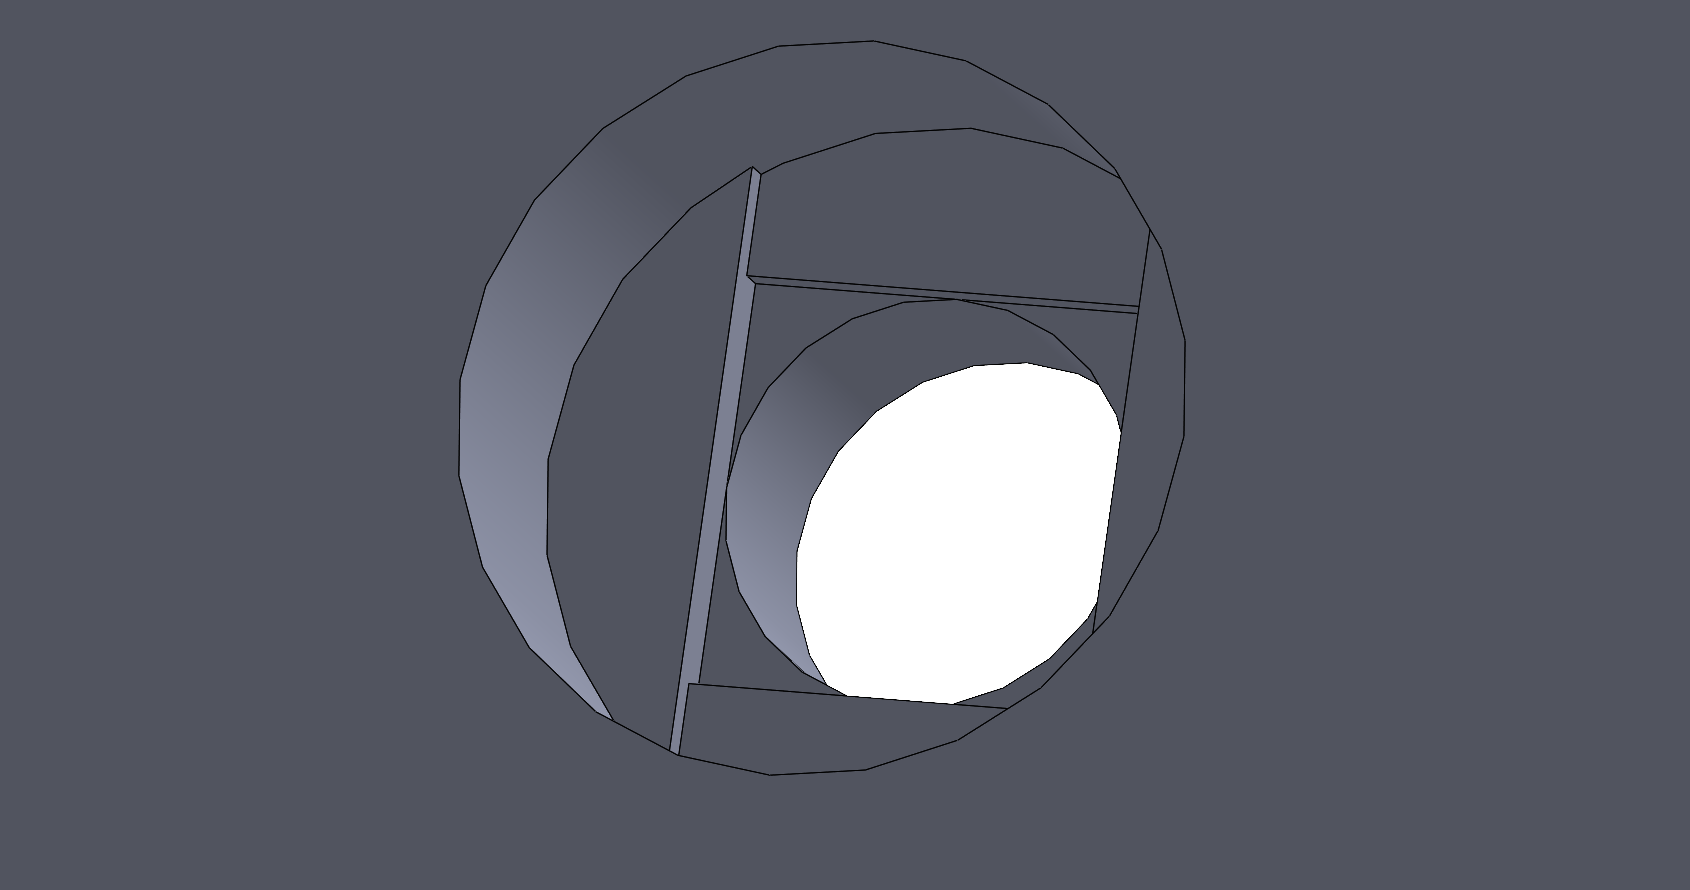
\includegraphics[width=0.5\linewidth]{screw_head_fitting}
	\caption{Design techniques used to avoid the need for support material}
	\label{fig:Screw head fitting}
\end{figure}
Different design techniques as shown in figure \ref{fig:Screw head fitting}were used specially for the place where the socket screws heads are inserted to avoid the need for support material.
\section{Assembly Process}
\subsection{Motors Assembly}
%the process of assembling the motors to be ready to be mounted on the chassis.
The hip and knee motors required assembly before they could be mounted on the chassis.
%%Two subfigures side by side of the hip_knee_motors_assembly and the horn_assembly_marking
\begin{figure}[h]
	\centering
	\begin{subfigure}[t]{0.45\textwidth}
		\centering
		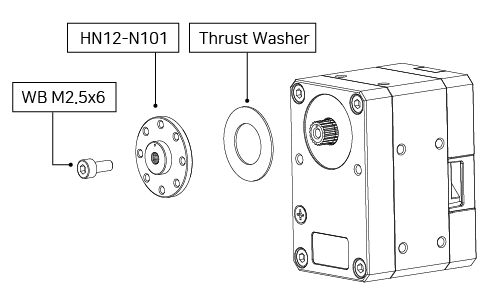
\includegraphics[height=0.7\textwidth]{hip_knee_motors_assembly}
		\caption{Hip and knee motors assembly}
		\label{fig:hipkneemotorsassembly}
	\end{subfigure}
	\begin{subfigure}[t]{0.45\textwidth}
		\centering
		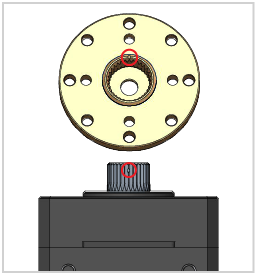
\includegraphics[height=0.7\textwidth]{horn_assembly_marking}
		\caption{Horn assembly marking}
		\label{fig:horn_assembly_marking}
	\end{subfigure}
	\caption{Comparison between the hip and knee motors assembly and the horn assembly marking}
	\label{fig:Comparison between the hip and knee motors assembly and the horn assembly marking}
\end{figure}

The assembly process is shown in figure \ref{fig:hipkneemotorsassembly} shows the normal horn assembly. the thrust washer should be placed between the horn and the motor to avoid friction between the horn and the motor. the horn should be tightened using the screw.As shown in figure \ref{fig:horn_assembly_marking} the indexing mark on the output horn is aligned with the index marking on the output shaft.

%figure for the motor spacer ring
\begin{figure}[h]
	\centering
	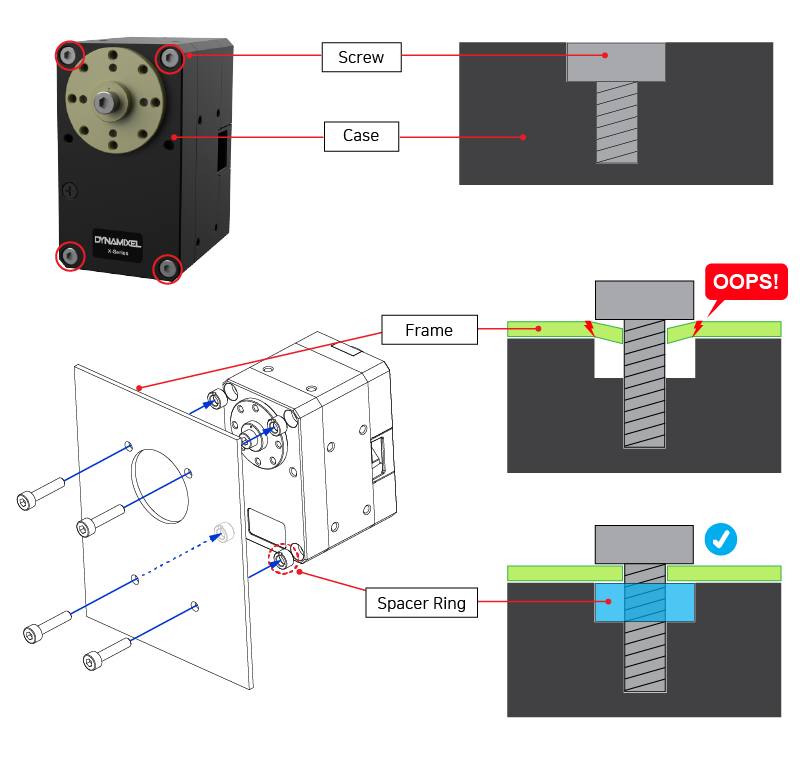
\includegraphics[width=0.5\linewidth]{motor_spacer_ring}
	\caption{Motor spacer ring}
	\label{fig:motorspacerring}
\end{figure}
The motor spacer ring shown in figure \ref{fig:motorspacerring} was used to make to fill the gap between the motor case and chassis frame.
The frame thickness was added to the length of the new screw to make sure that the screw is not larger than the depth of the mounting point or the motor case may be damaged.

\subsection{Screws and thread inserts}
The screws and thread inserts used in the assembly are shown in the table \ref{tab:screws}.
The precise dimensions of the screws and thread inserts were important to make sure that the assembly process goes smoothly.
The tolerance of 0.1 mm for the screws was acceptable for the assembly process except for the screws used for the hip and knee motors horns as it could touch the thrust washer and cause damage to the motor.

%table for the screws and thread inserts used in the assembly
\begin{table}[h!]
	\centering
	\caption{Screws and thread inserts used in the assembly}
	\label{tab:screws}
	\begin{tabular}{lcl}
		\toprule
		Component & Quantity & Screw size \\
		\midrule
		Wheel Motor & 8 & M3*8 \\
		Knee Motor Horn & 16 & M2*13 \\
		Knee Motor front & 8 & M2.5*14 \\
		Knee Motor Top & 8 & M2.5*5 \\
		Knee Motor sides & 20 & M2.5*5 or M2.5*5 .5 \\
		Hip Motor front & 8 & M2.5*6 \\
		Hip Motor Horn & 16 & M2*15 \\
		Hip Motor side & 8 & M2.5*15 \\
		Body & 12 & M2.5*6 \\
		Wheel Motor cover & 20 & M2.5*6 \\
		Thread inserts & 36 & M2.5 x 5.7 \\
		\bottomrule
	\end{tabular}
\end{table}


%\ref{tab:screws}.
\subsection{Chassis Assembly}
%figure for the assembled chassis
\begin{figure}[h]
	\centering
	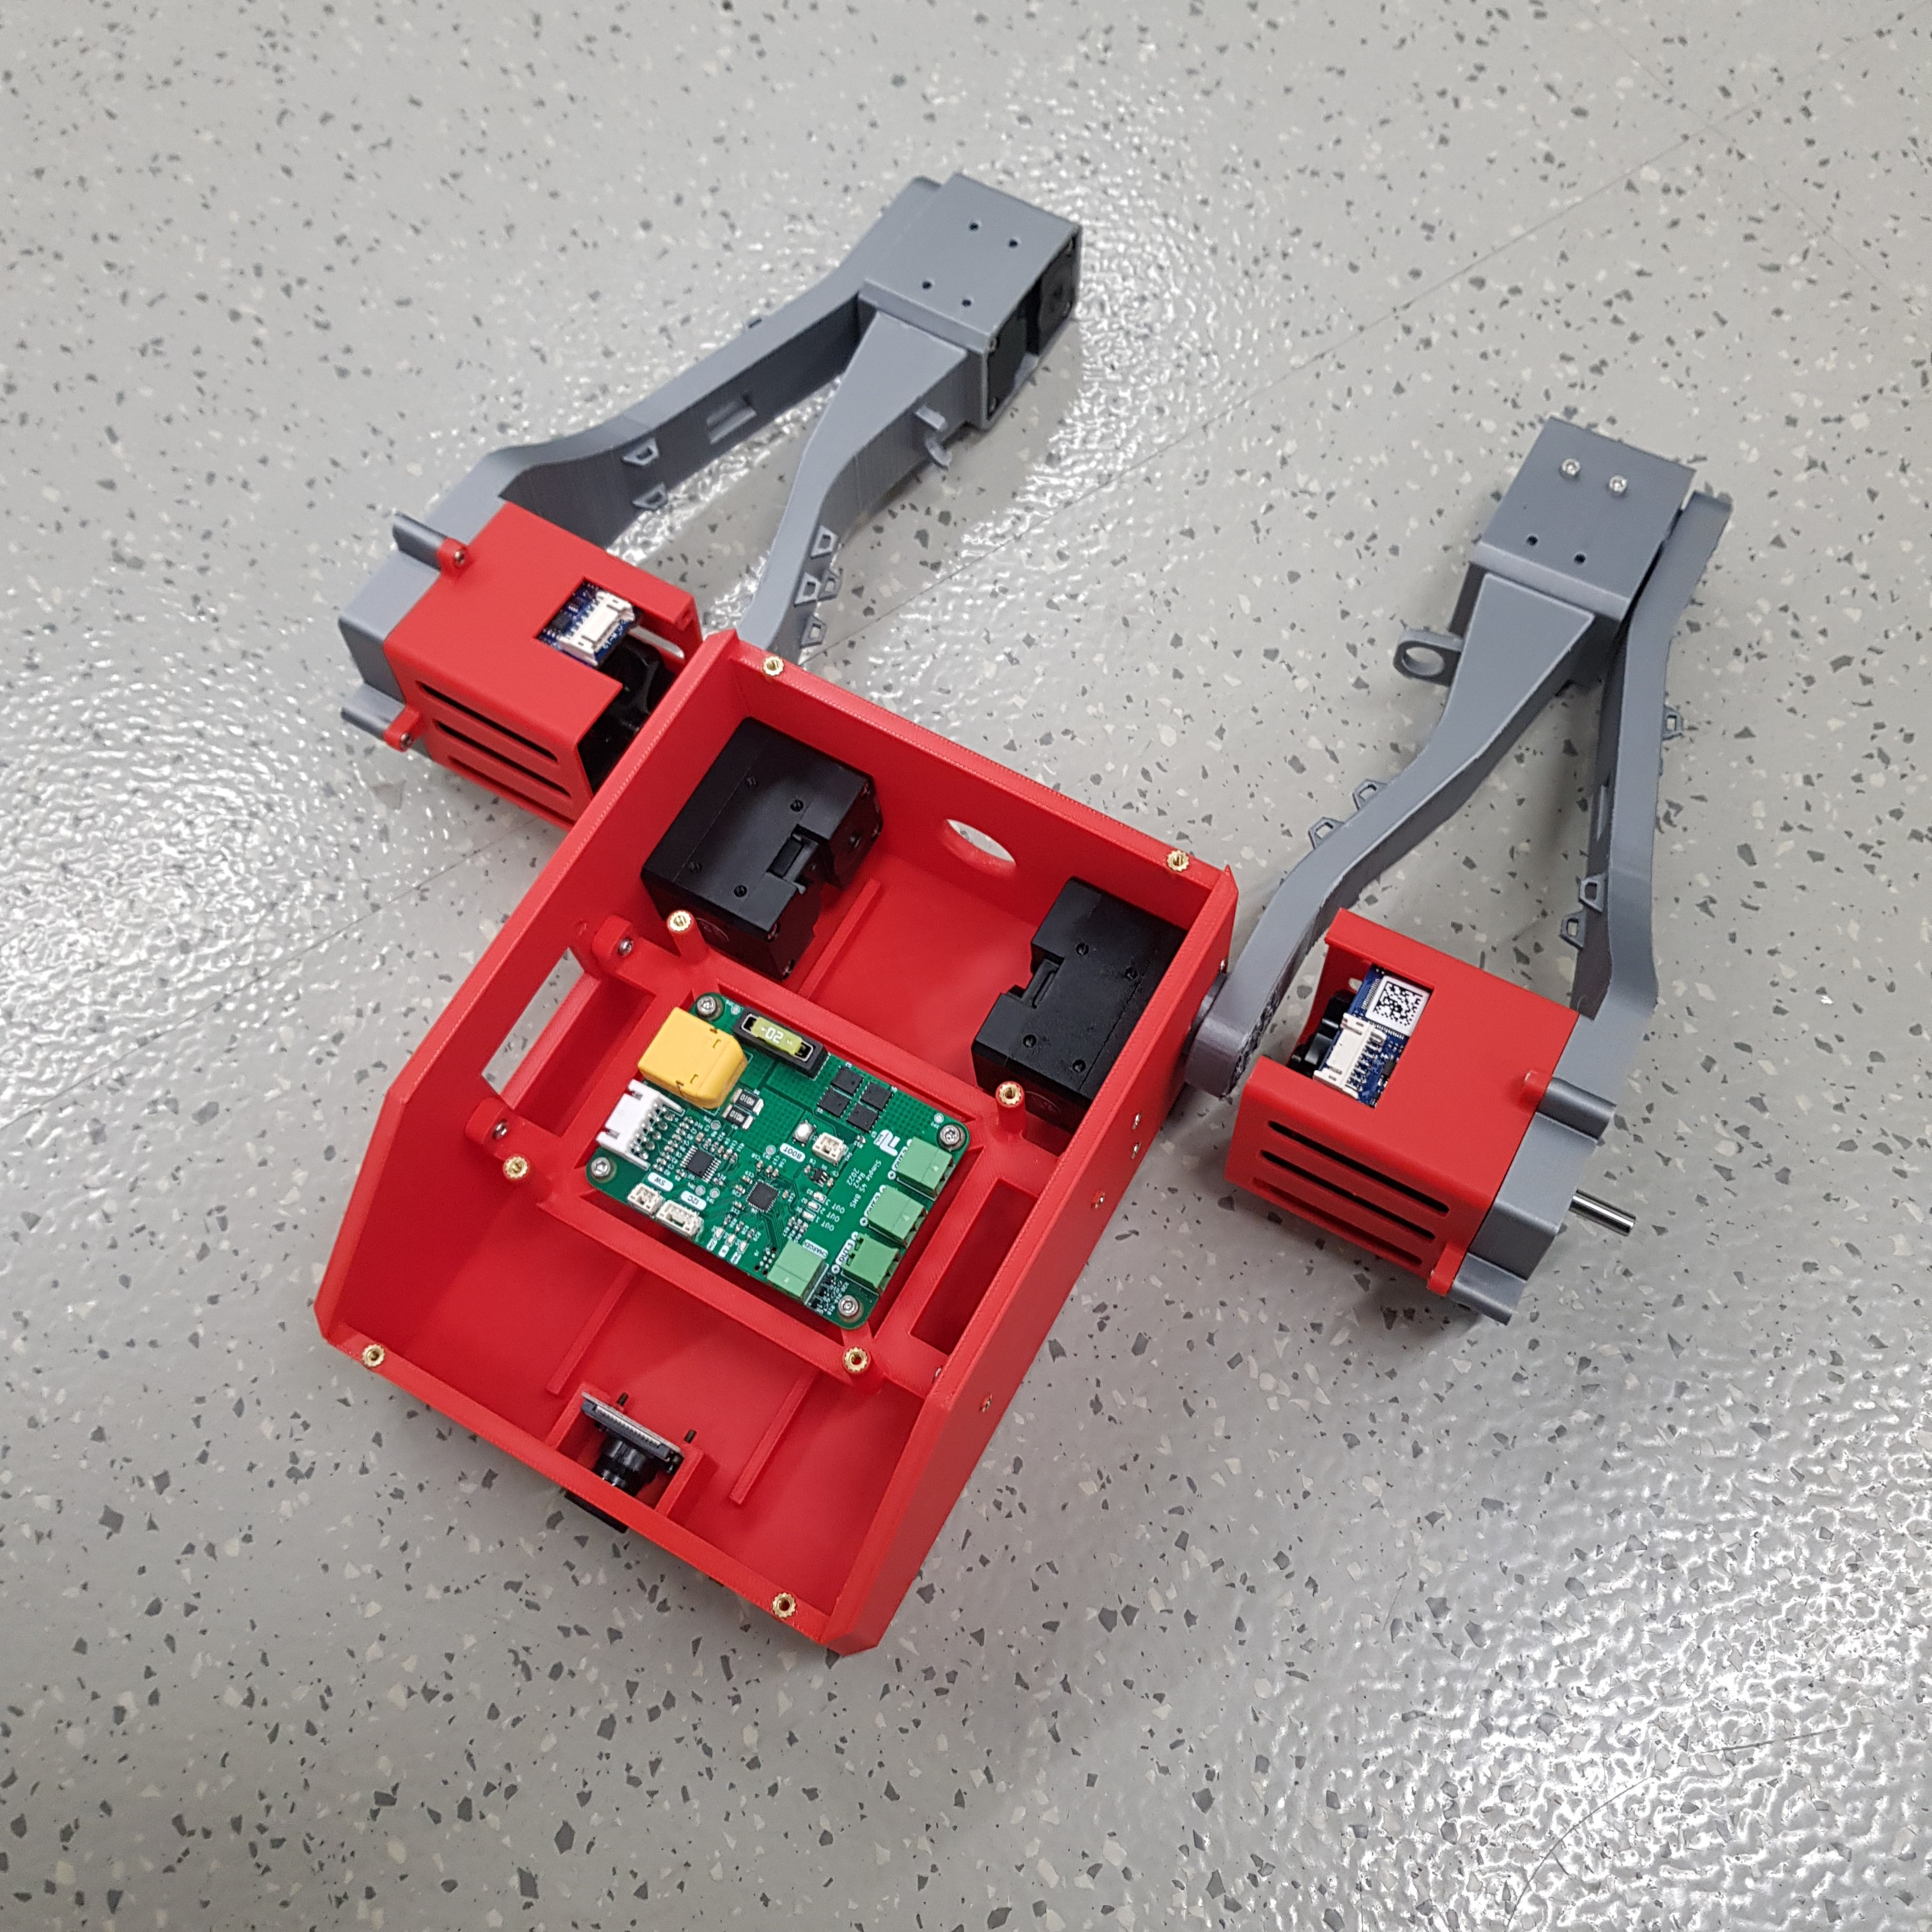
\includegraphics[width=0.5\linewidth]{chassis_assembled}
	\caption{Assembled chassis}
	\label{fig:chassisassembled}
\end{figure}
%\begin{itemize}
%\item Step-by-step explanation of the assembly process.
The assembly process started with the chassis, the chassis was assembled using screws and thread inserts.
First the thread inserts were inserted into the chassis using soldering iron, then the screws were used to assemble the motors to the knee wheel links, the hip knee links, the body.
then the knee wheel links were assembled to the hip knee links

%\item Tools and techniques used in the assembly.
%\item Assembly sequence and rationale behind it.
%\end{itemize}
\newpage
%several figures for the assembly process of the chassis
%three subfigures for the thread inserts (Body thread inserts, knee wheel link thread inserts, Board mounting rack thread inserts)
\begin{figure}[h]
	\centering
	\begin{subfigure}[t]{0.3\textwidth}
		\centering
		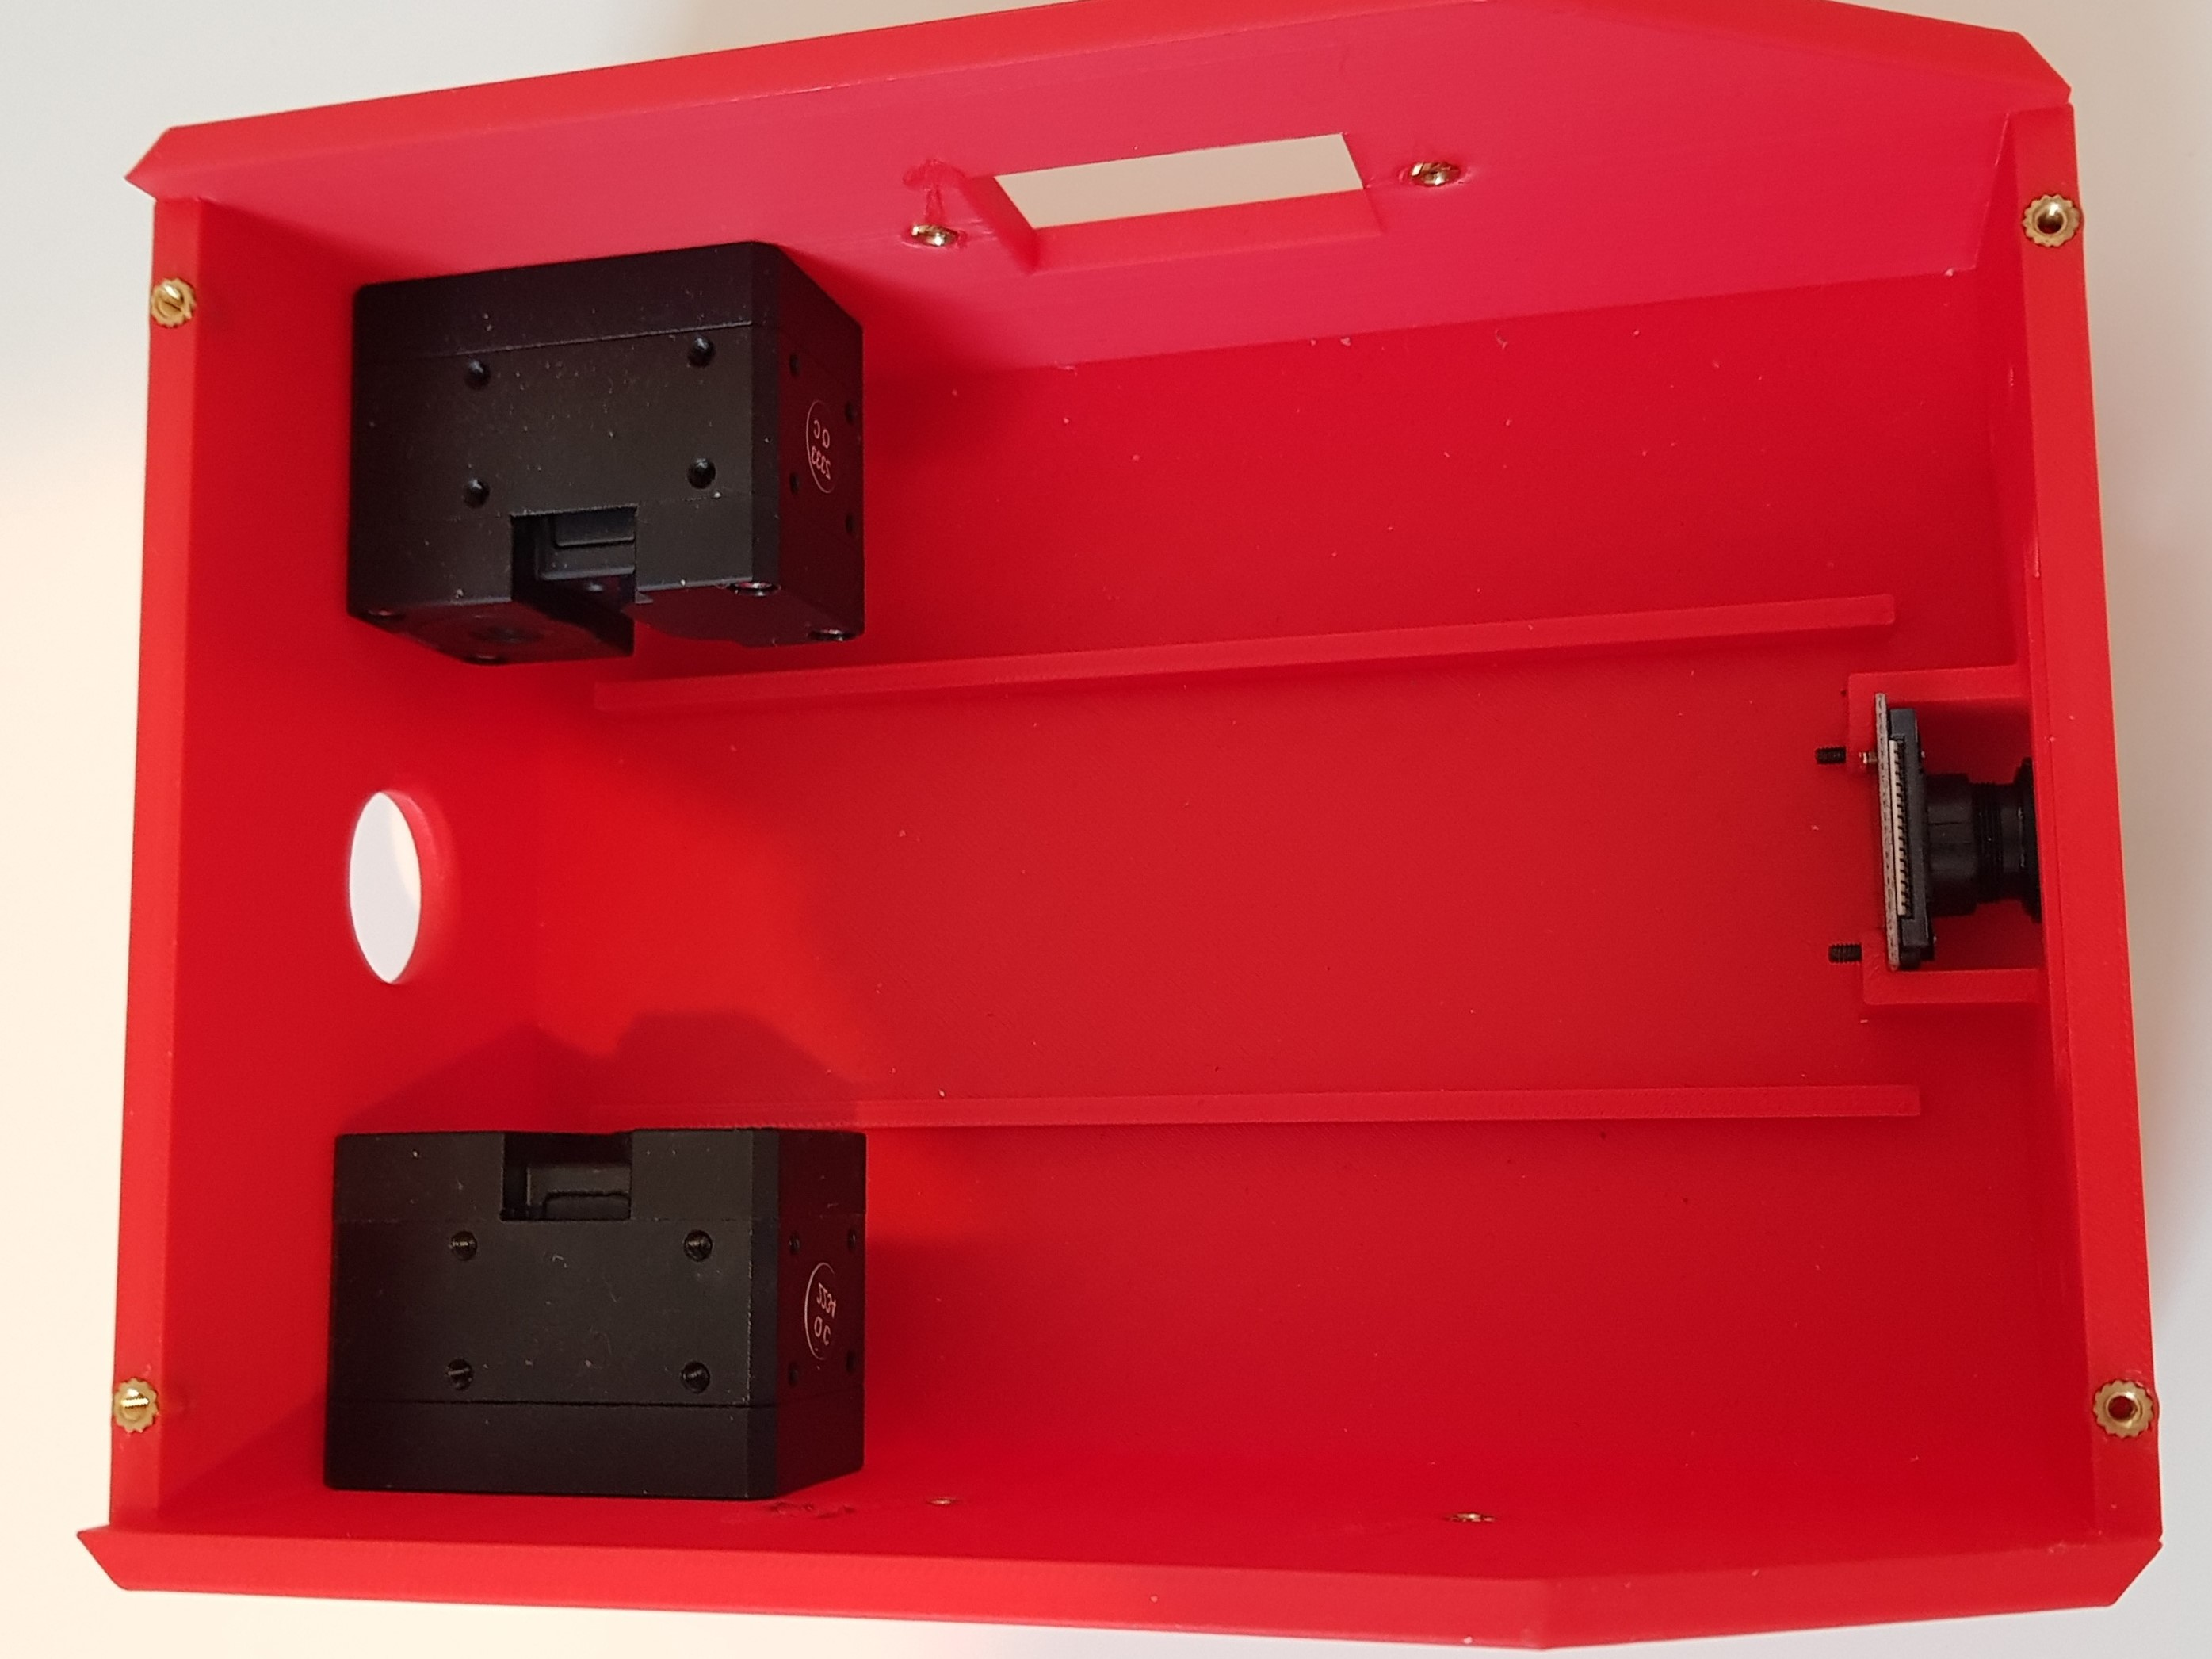
\includegraphics[height=0.7\textwidth]{body_thread_inserts}
		\caption{Body thread inserts}
		\label{fig:bodythreadinserts}
	\end{subfigure}
	\begin{subfigure}[t]{0.3\textwidth}
		\centering
		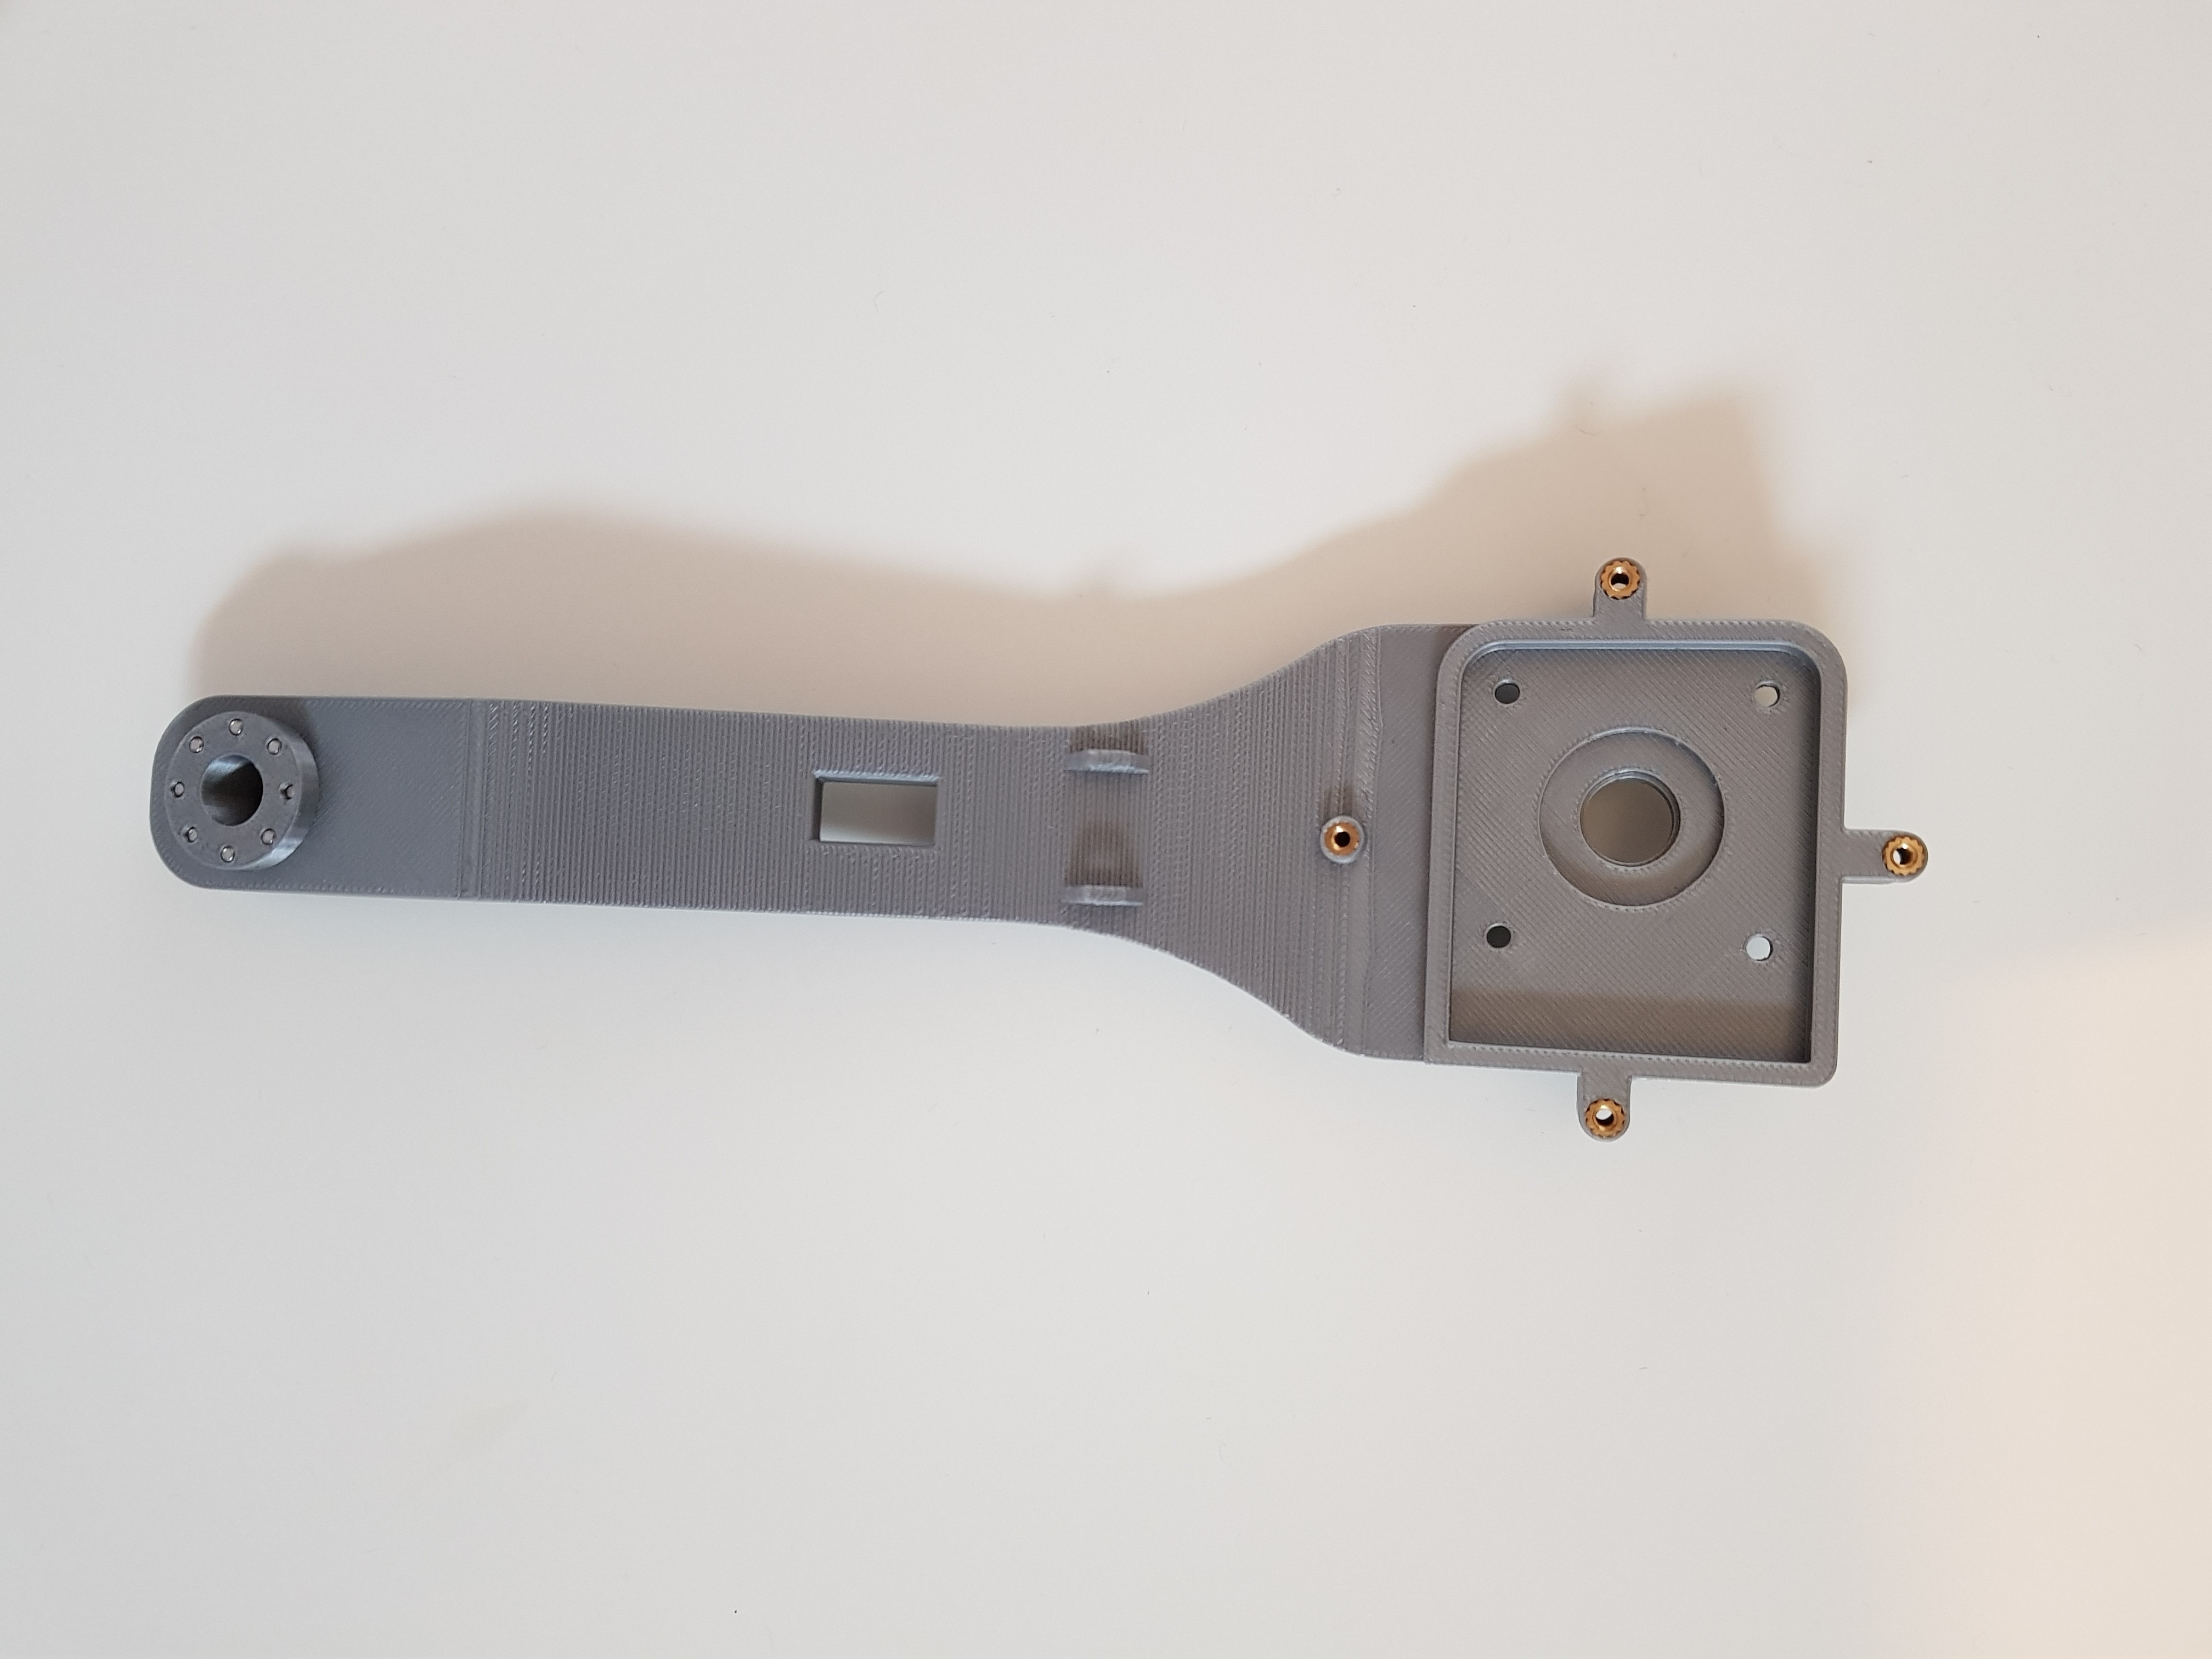
\includegraphics[height=0.7\textwidth]{knee_wheel_link_thread_inserts}
		\caption{Knee wheel link thread inserts}
		\label{fig:kneewheellinkthreadinserts}
	\end{subfigure}
	\begin{subfigure}[t]{0.3\textwidth}
		\centering
		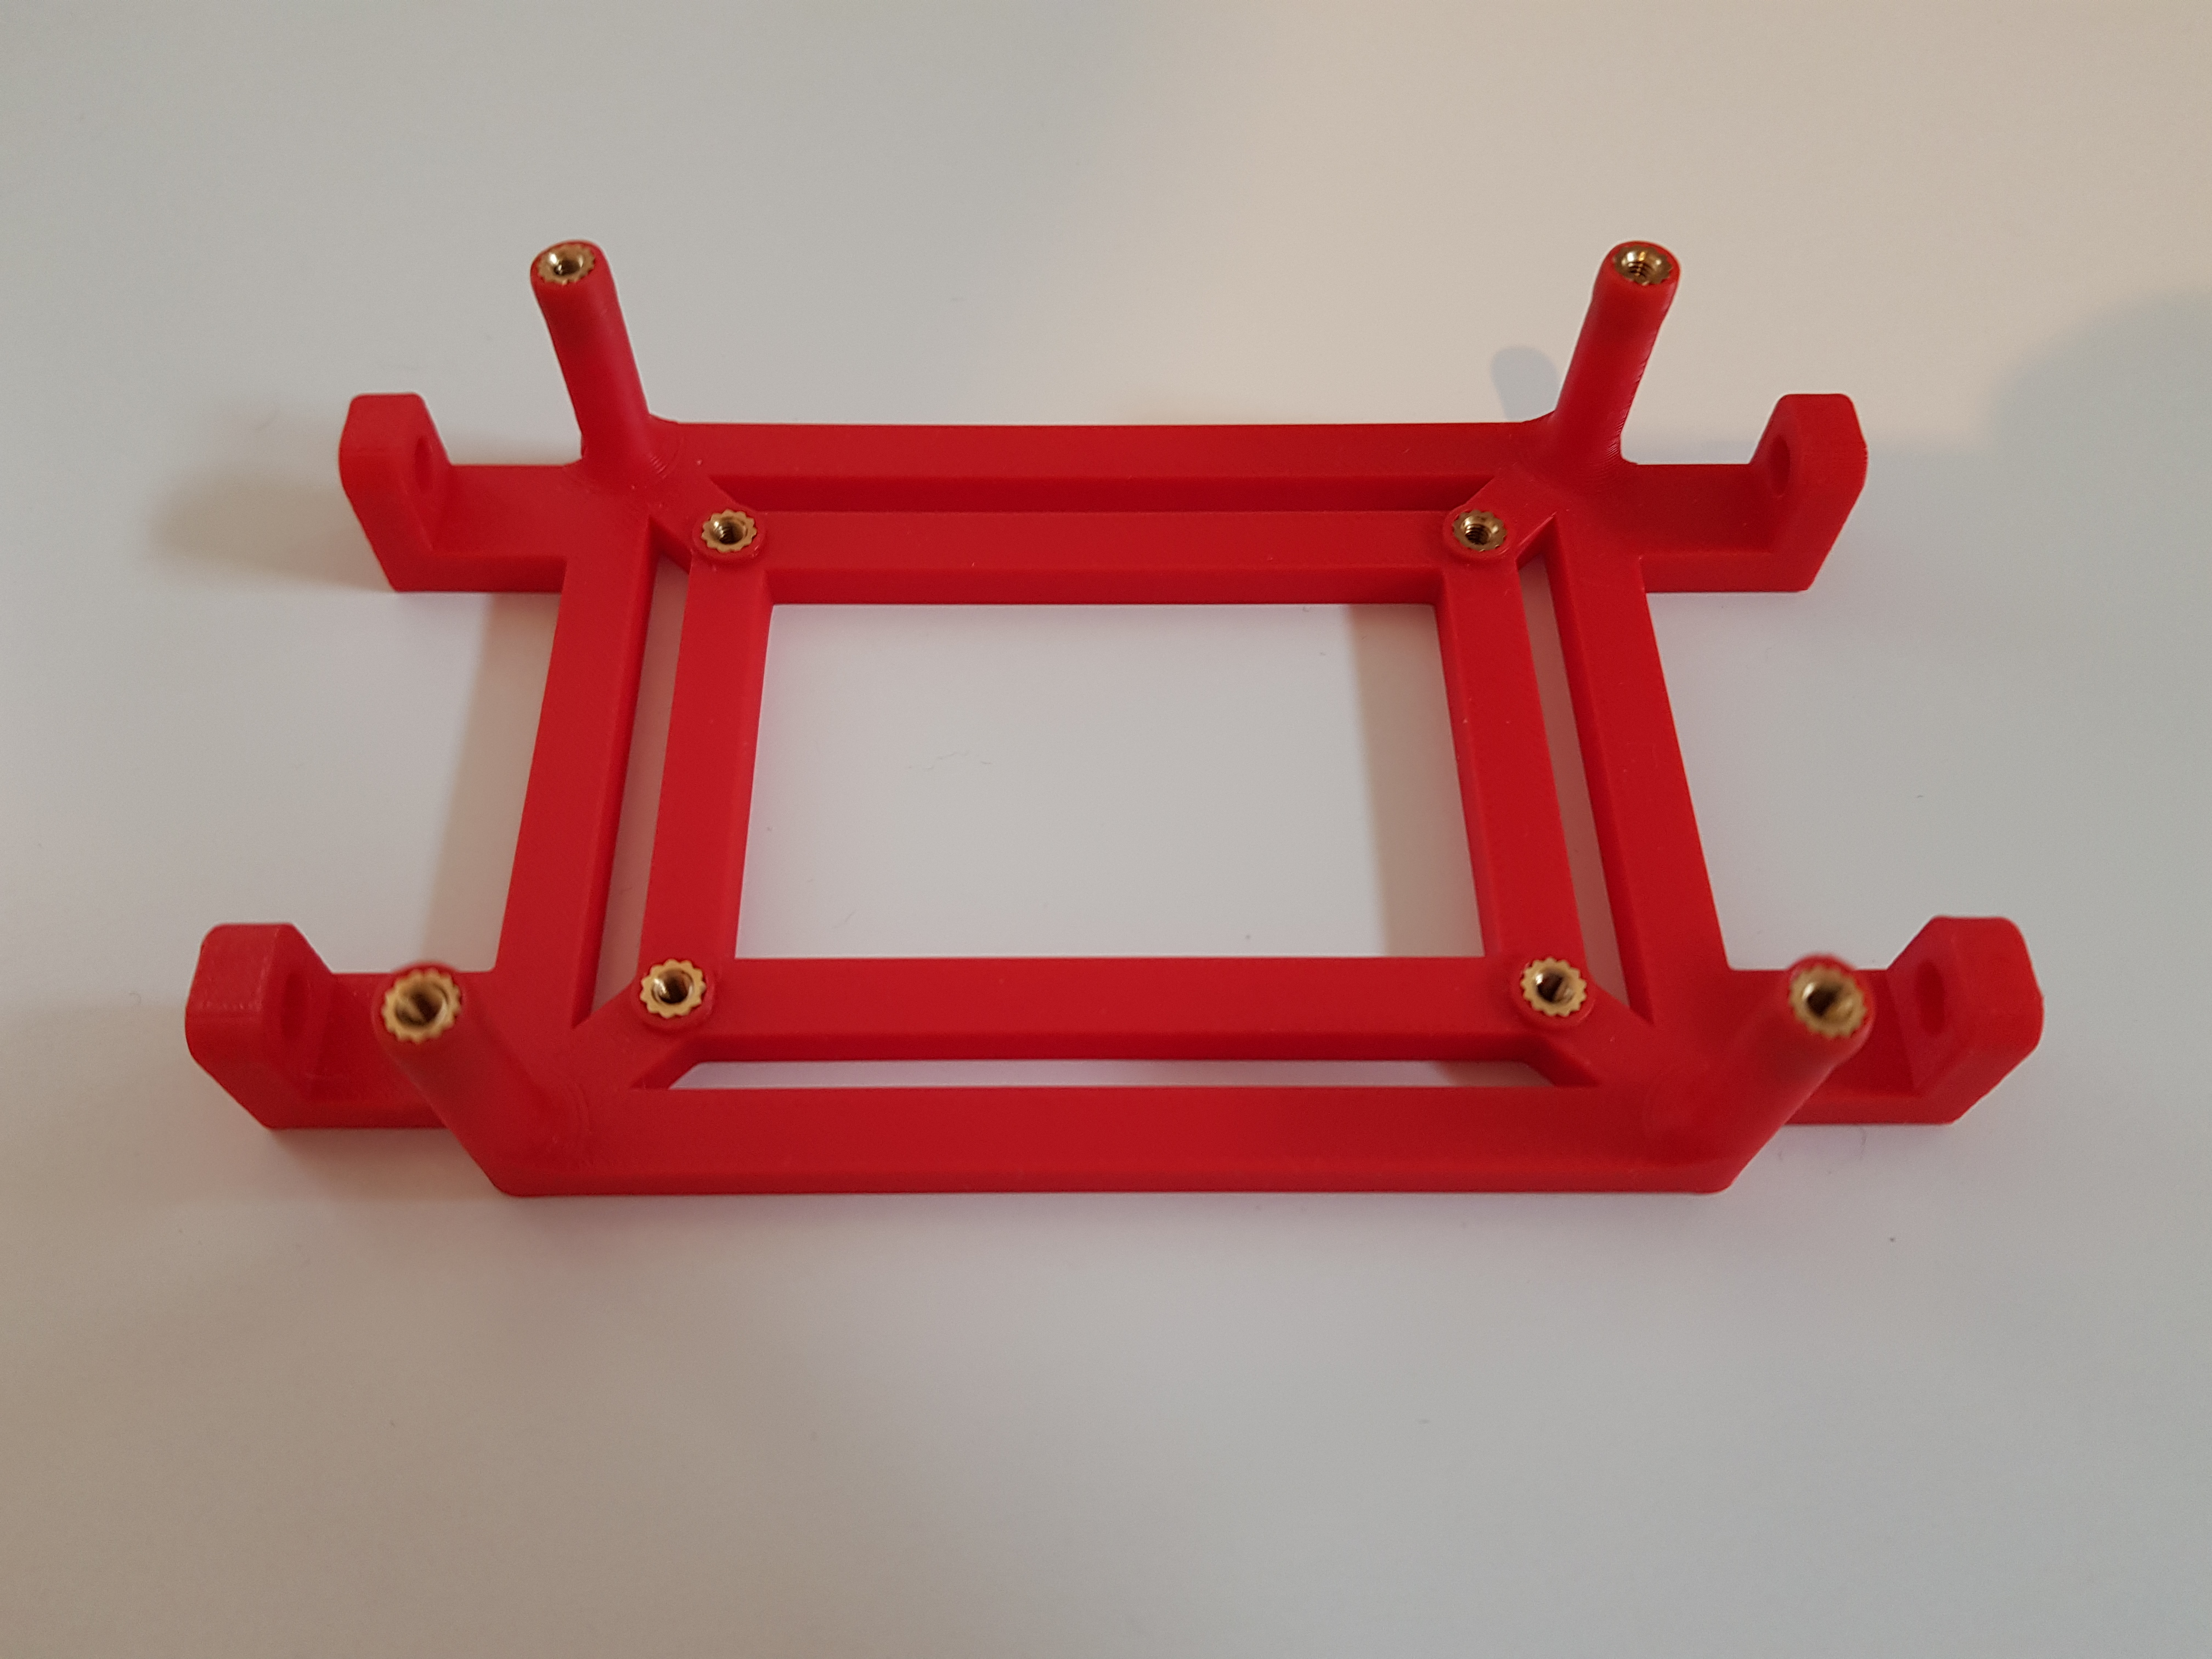
\includegraphics[height=0.7\textwidth]{board_mounting_rack_thread_inserts}
		\caption{Board mounting rack thread inserts}
		\label{fig:boardmountingrackthreadinserts}
	\end{subfigure}
	\caption{Thread inserts}
	\label{fig:Thread inserts}
\end{figure}

The thread inserts were inserted into the chassis using a soldering iron as shown in figure \ref{fig:Thread inserts} for the body, knee wheel links and the board mounting rack.
Minimum force was applied to the soldering iron to align the thread inserts surface with the surface of the chassis.
%two subfigures for mounting the motors on the knee wheel links
\begin{figure}[h]
	\centering
	\begin{subfigure}[t]{0.45\textwidth}
		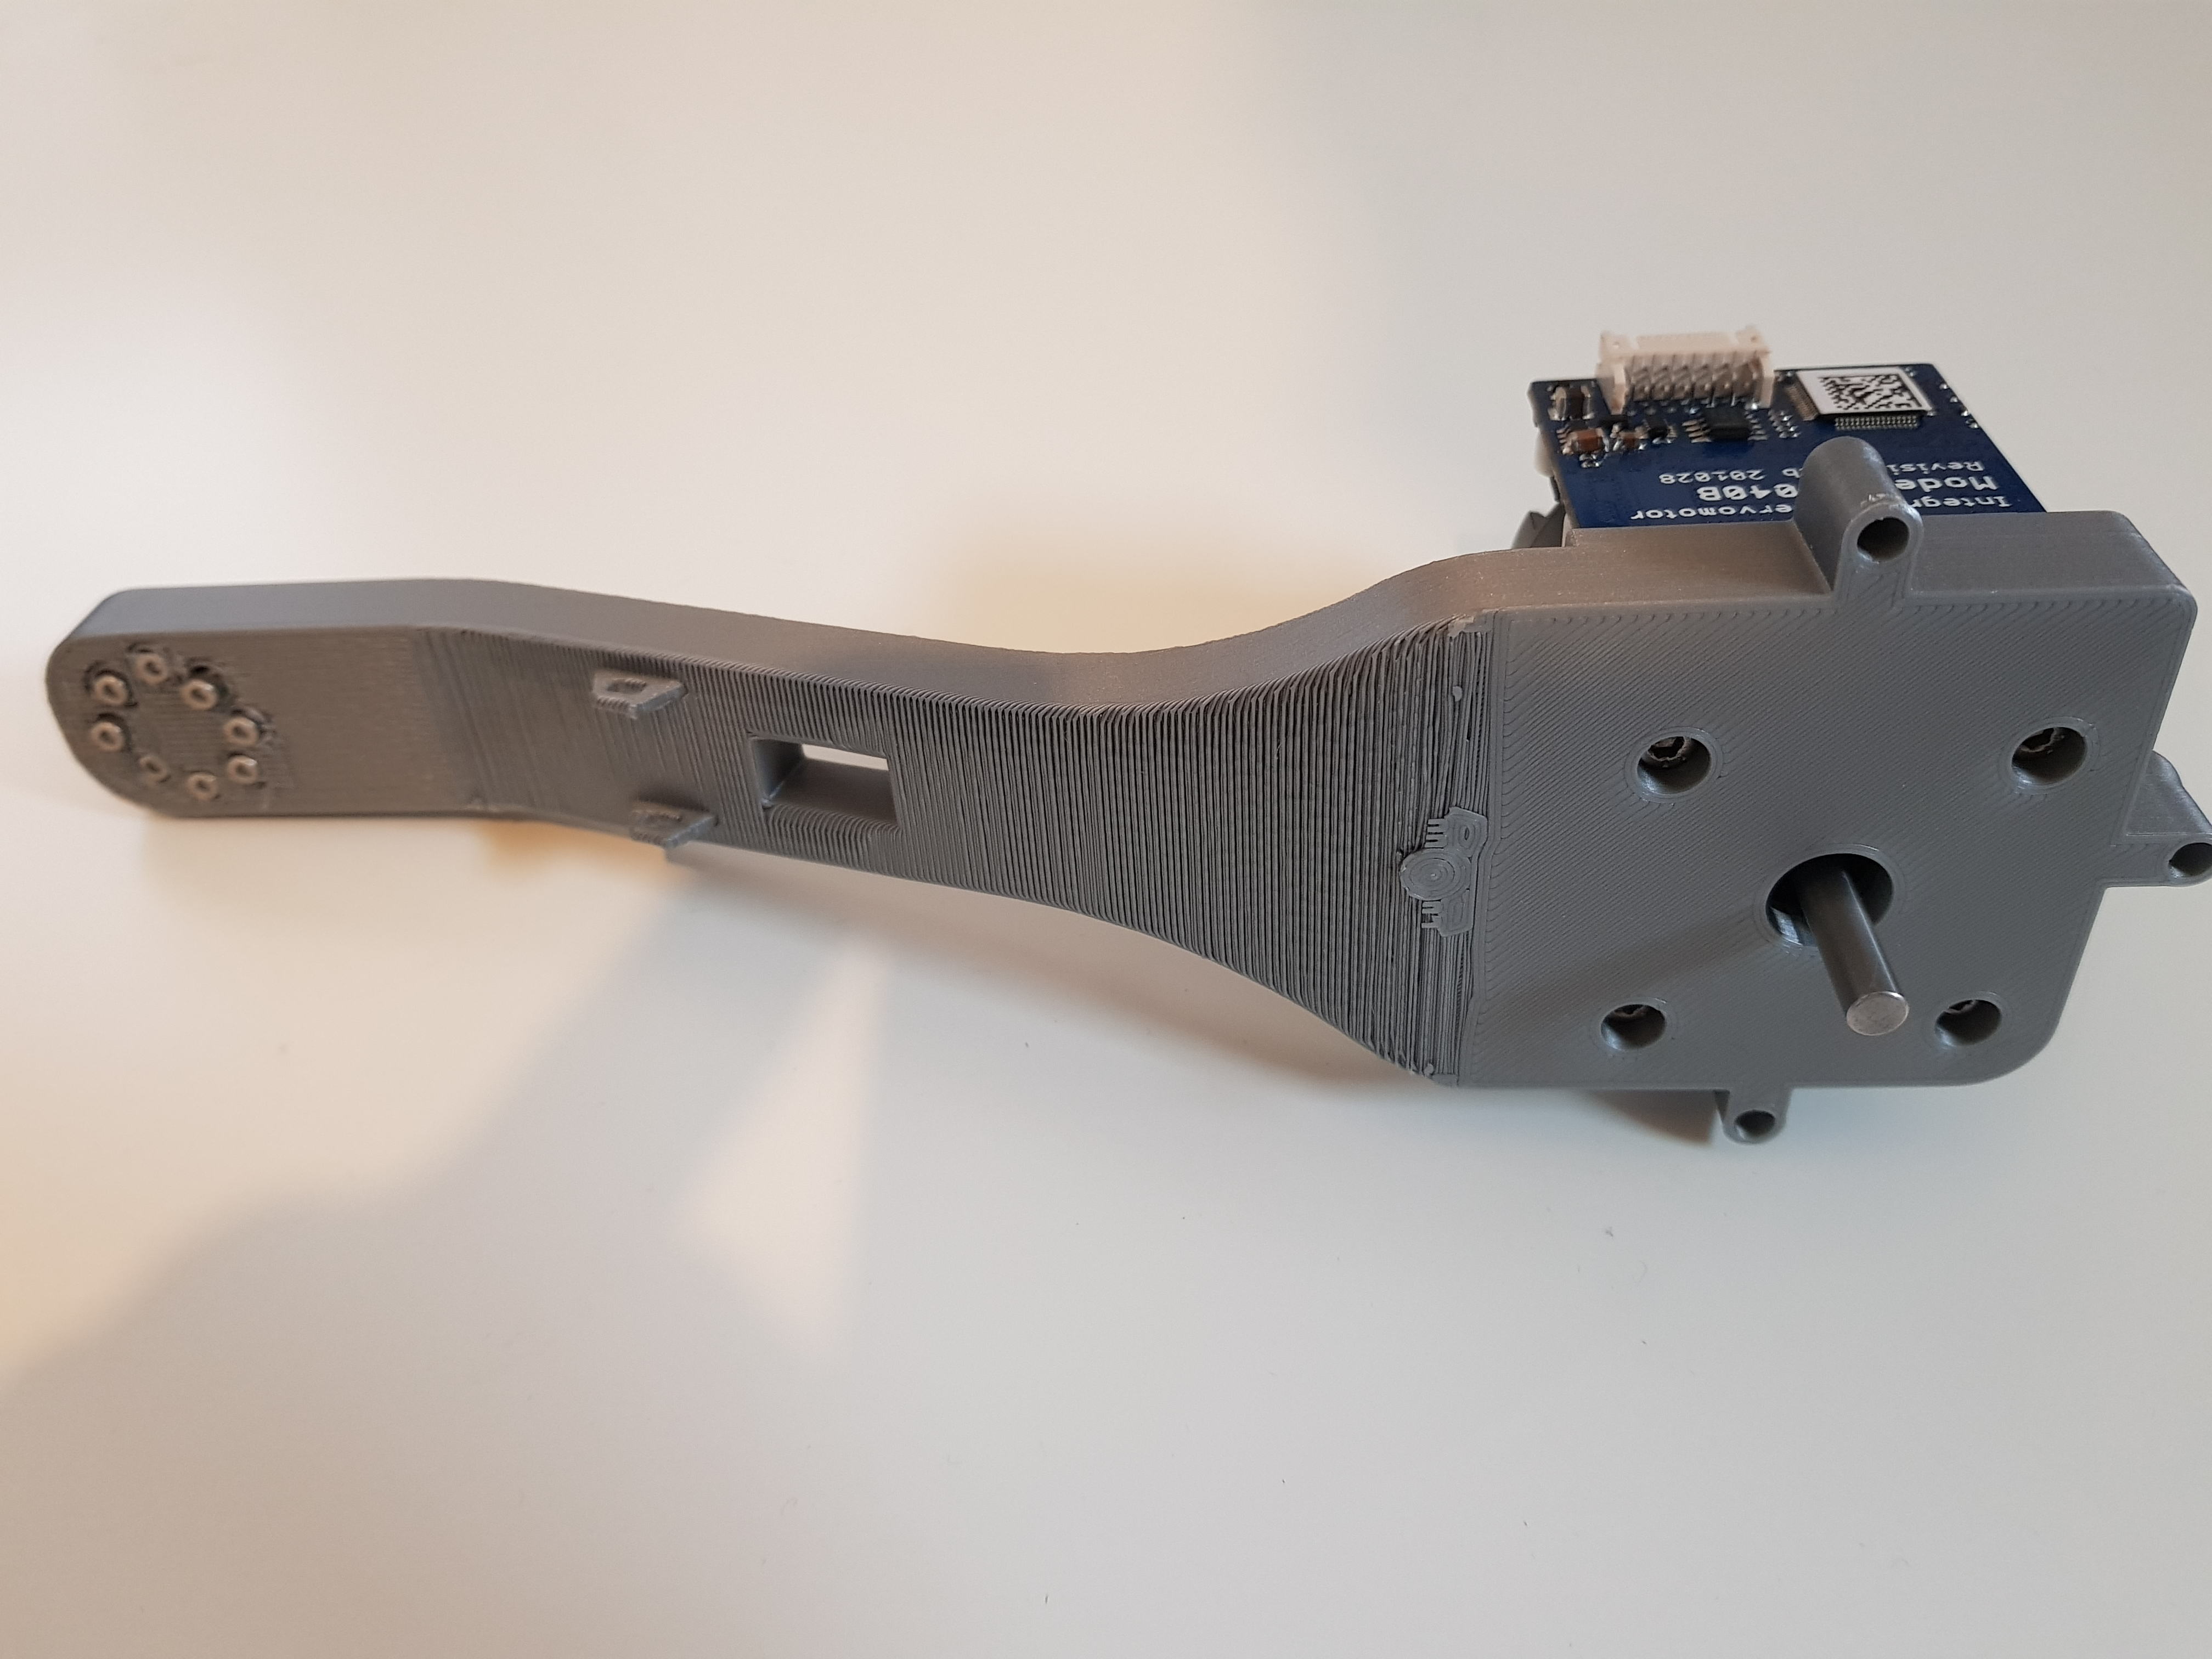
\includegraphics[height=0.7\textwidth]{mounting_motors_on_knee_wheel_links_1}
		\caption{Mounting motors on knee wheel links perspective view}
		\label{fig:mountingmotorsonkneewheellinksperpectiveview}
	\end{subfigure}
	\begin{subfigure}[t]{0.45\textwidth}
		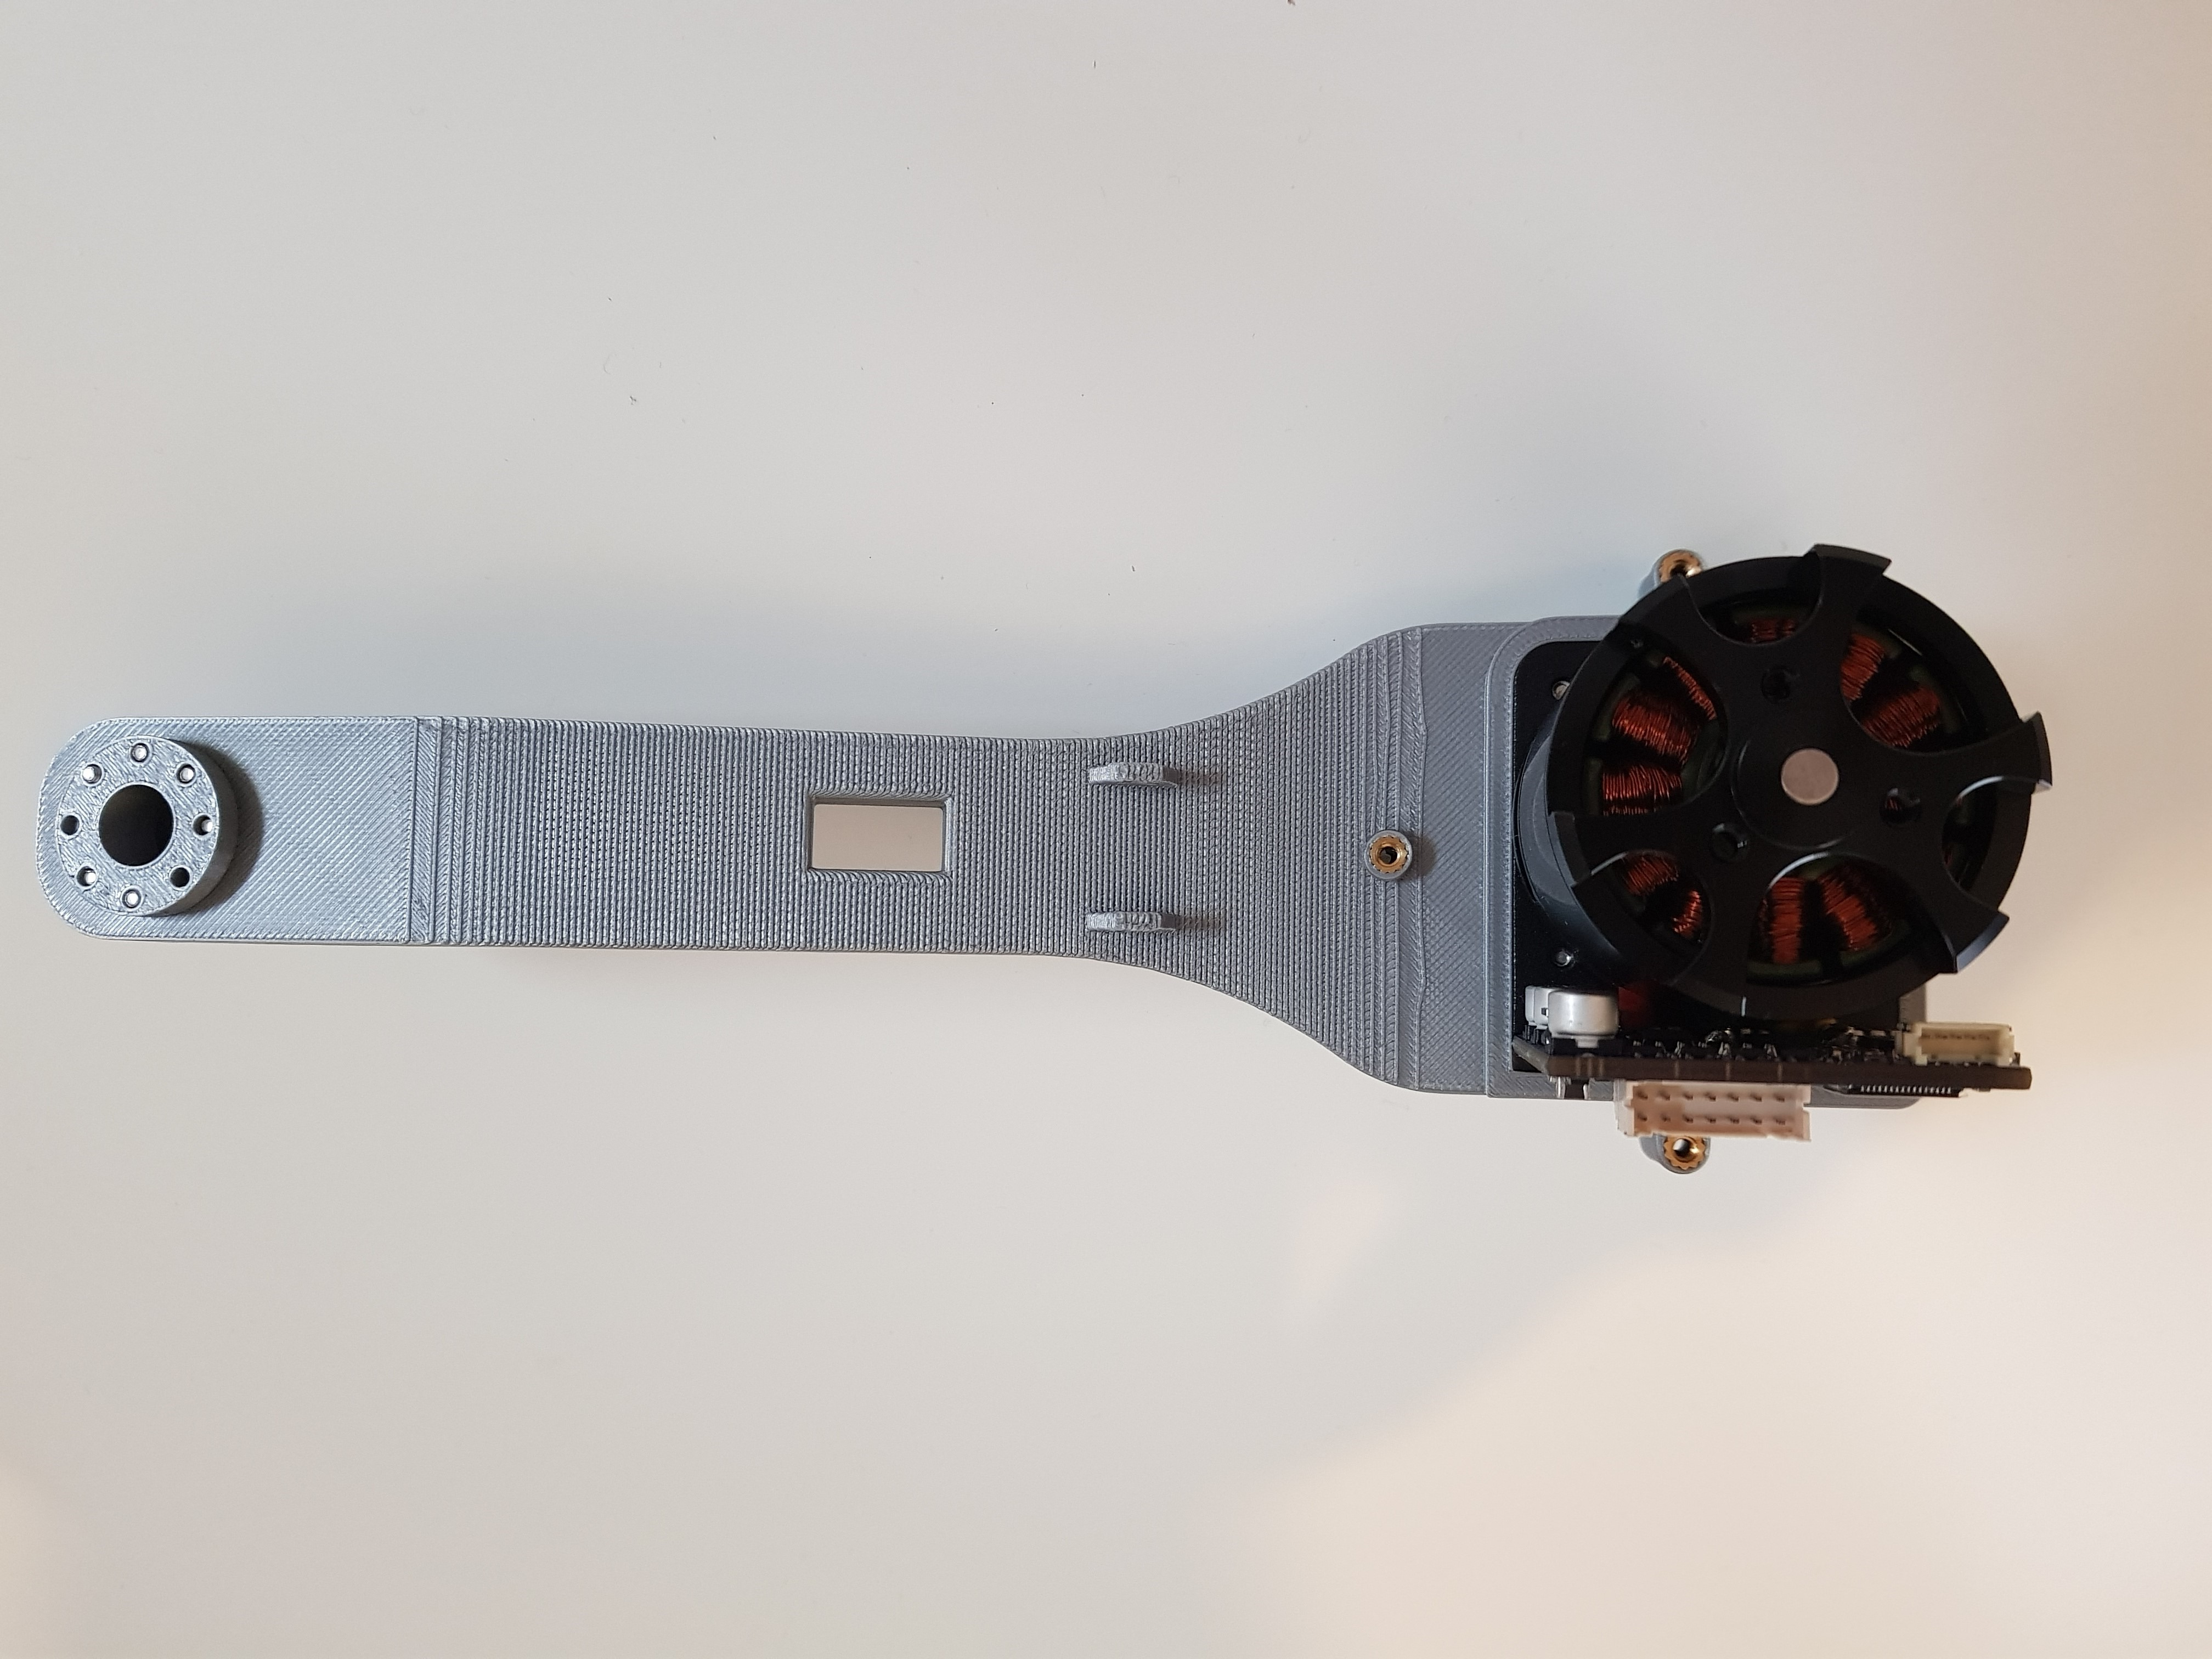
\includegraphics[height=0.7\textwidth]{mounting_motors_on_knee_wheel_links_2}
		\caption{Mounting motors on knee wheel links top view}
		\label{fig:mountingmotorsonkneewheellinkstopview}
	\end{subfigure}
	\caption{Mounting motors on knee wheel links}
	\label{fig:Mounting motors on knee wheel links}
\end{figure}
%%figure for mounting the motors on the knee wheel links
%\begin{figure}[h]
%	\centering
%	\includegraphics[width=0.5\linewidth]{mounting_motors_on_knee_wheel_links}
%	\caption{Mounting motors on knee wheel links}
%	\label{fig:mountingmotorsonkneewheellinks}
%\end{figure}

The wheel motors were mounted on the knee wheel links using four screws, as shown in figure \ref{fig:mountingmotorsonkneewheellinks}. The SC040B aluminum extrusion that holds the motor and electronics allows the motor to be mounted on the knee wheel links. free moving air around the motor is important to keep the motor cool and to avoid overheating.
%two subfigures for mounting the motors on the hip knee links
\begin{figure}[h]
	\centering
	\begin{subfigure}[t]{0.45\textwidth}
		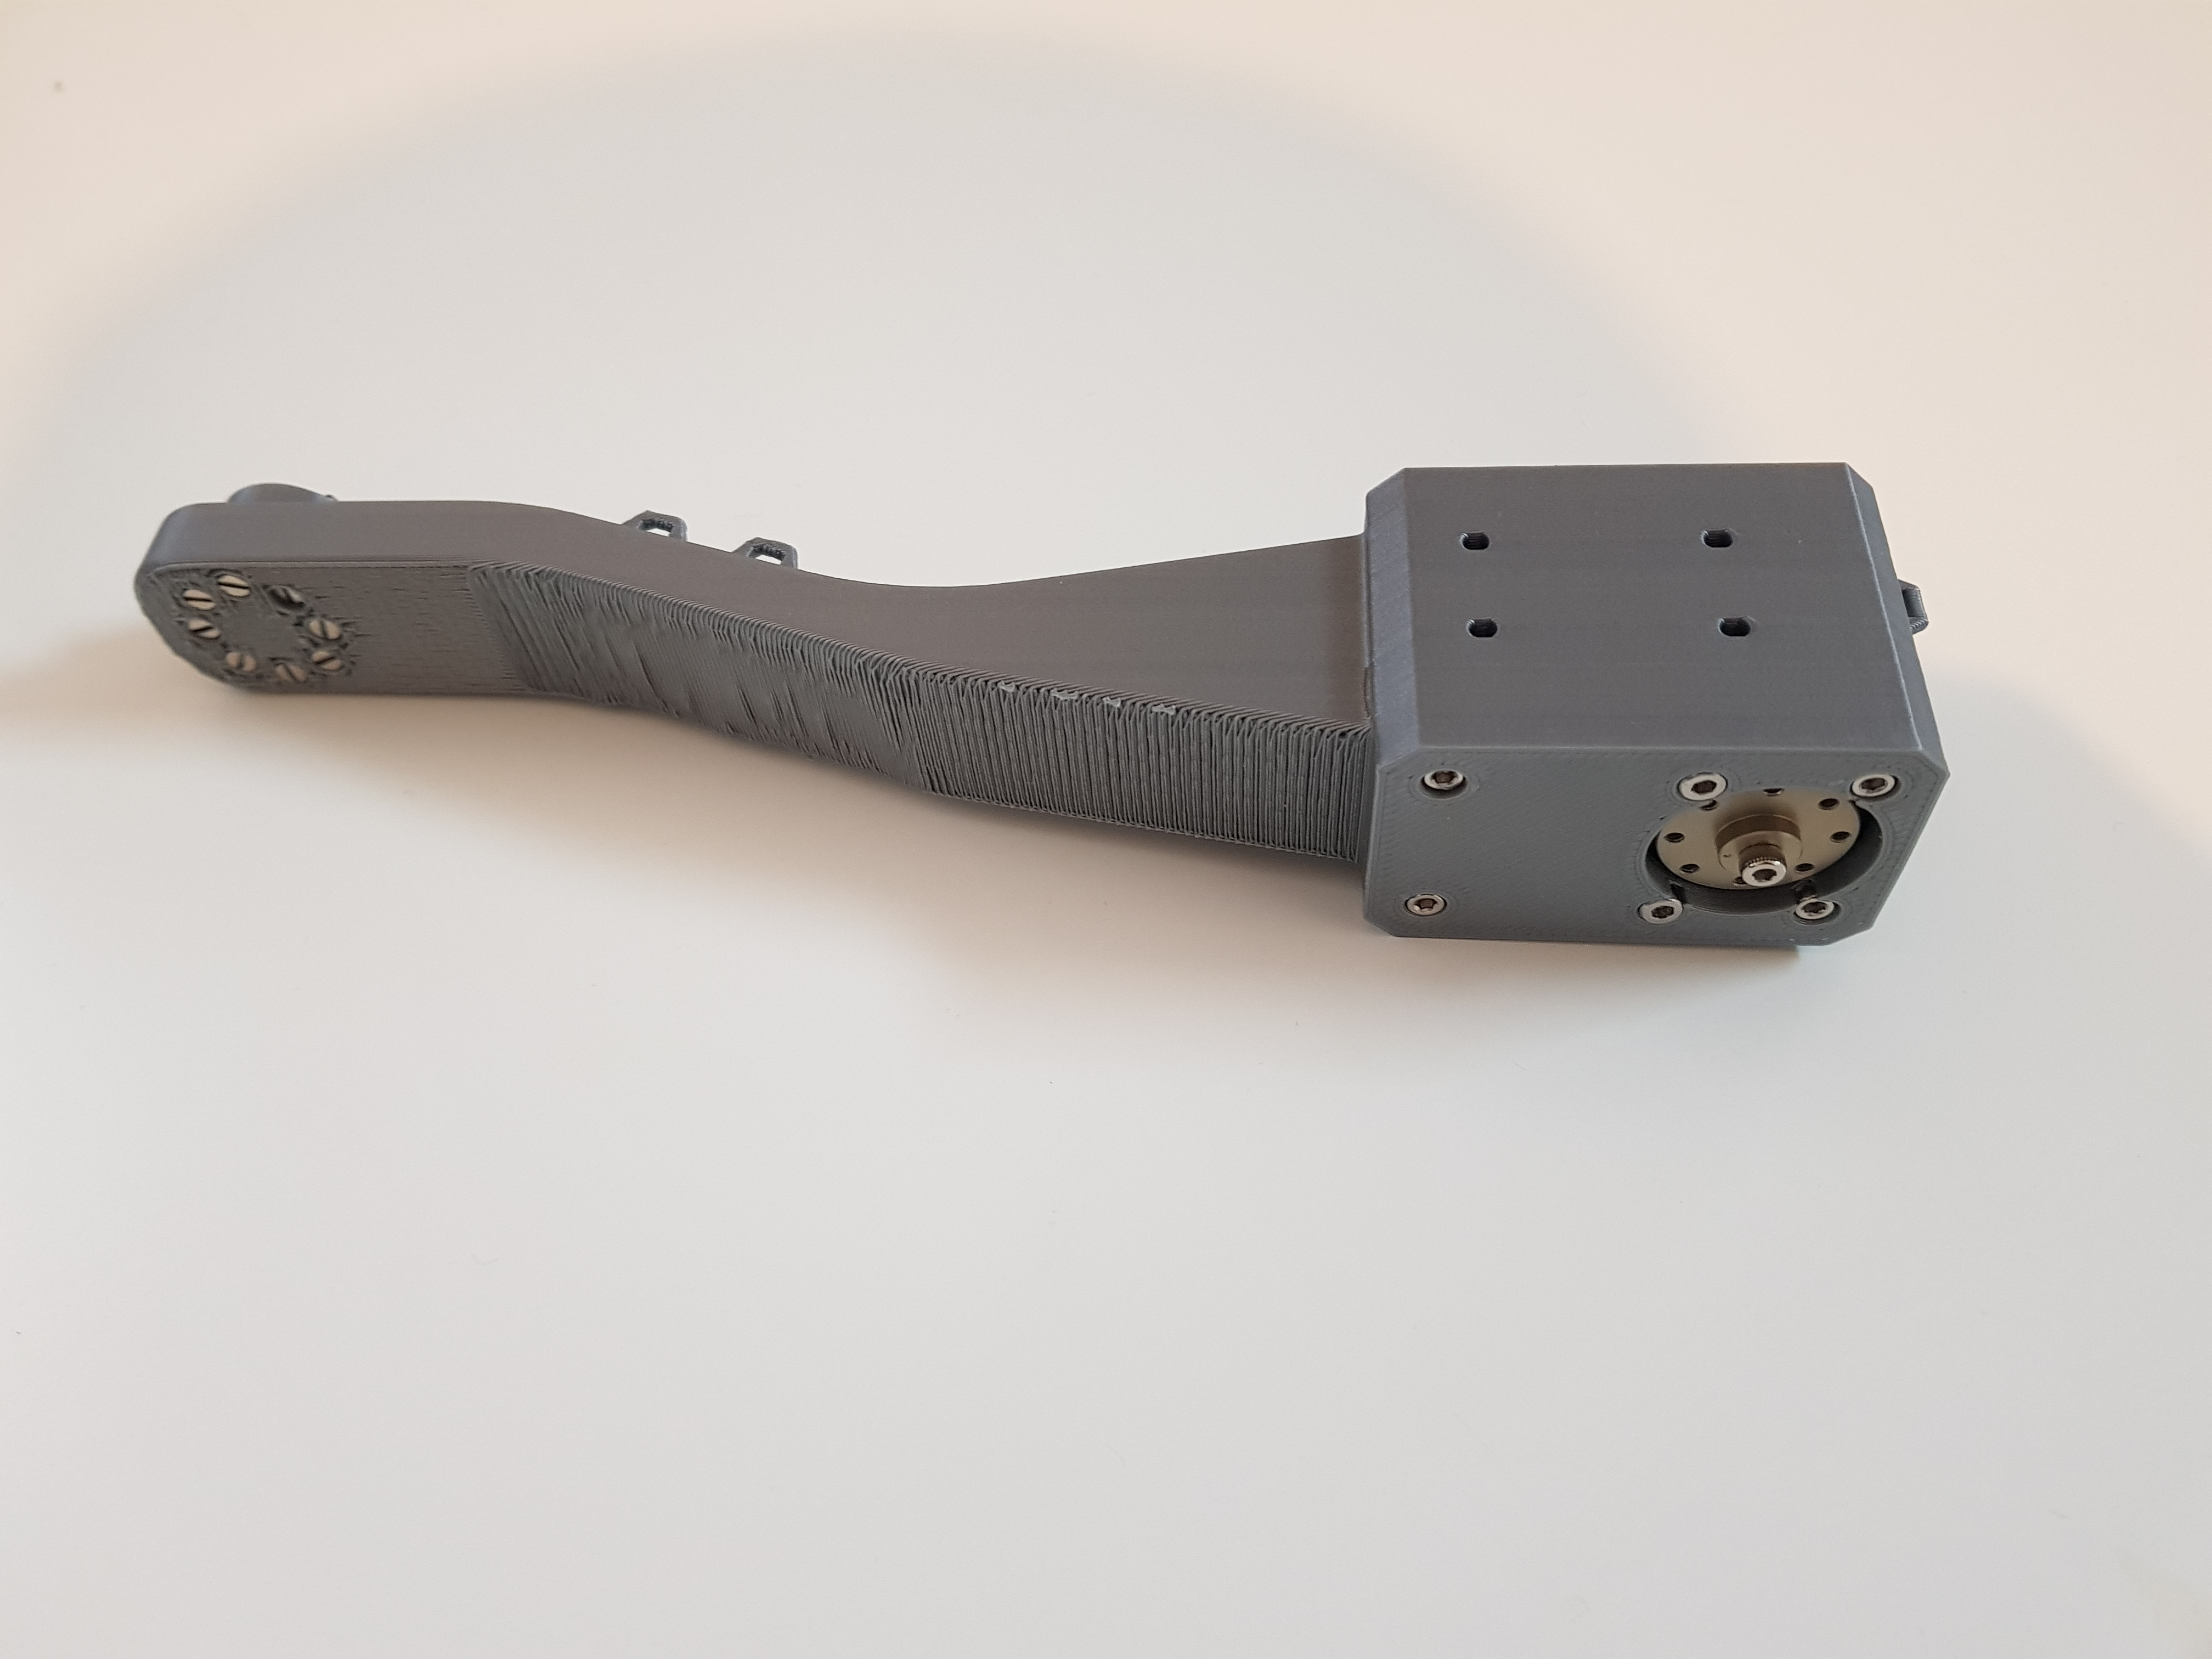
\includegraphics[height=0.7\textwidth]{mounting_motors_on_hip_knee_links_1}
		\caption{Mounting motors on hip knee links perspective view}
		\label{fig:mountingmotorsonhipkneelinksperspectiveview}
	\end{subfigure}
	\begin{subfigure}[t]{0.45\textwidth}
		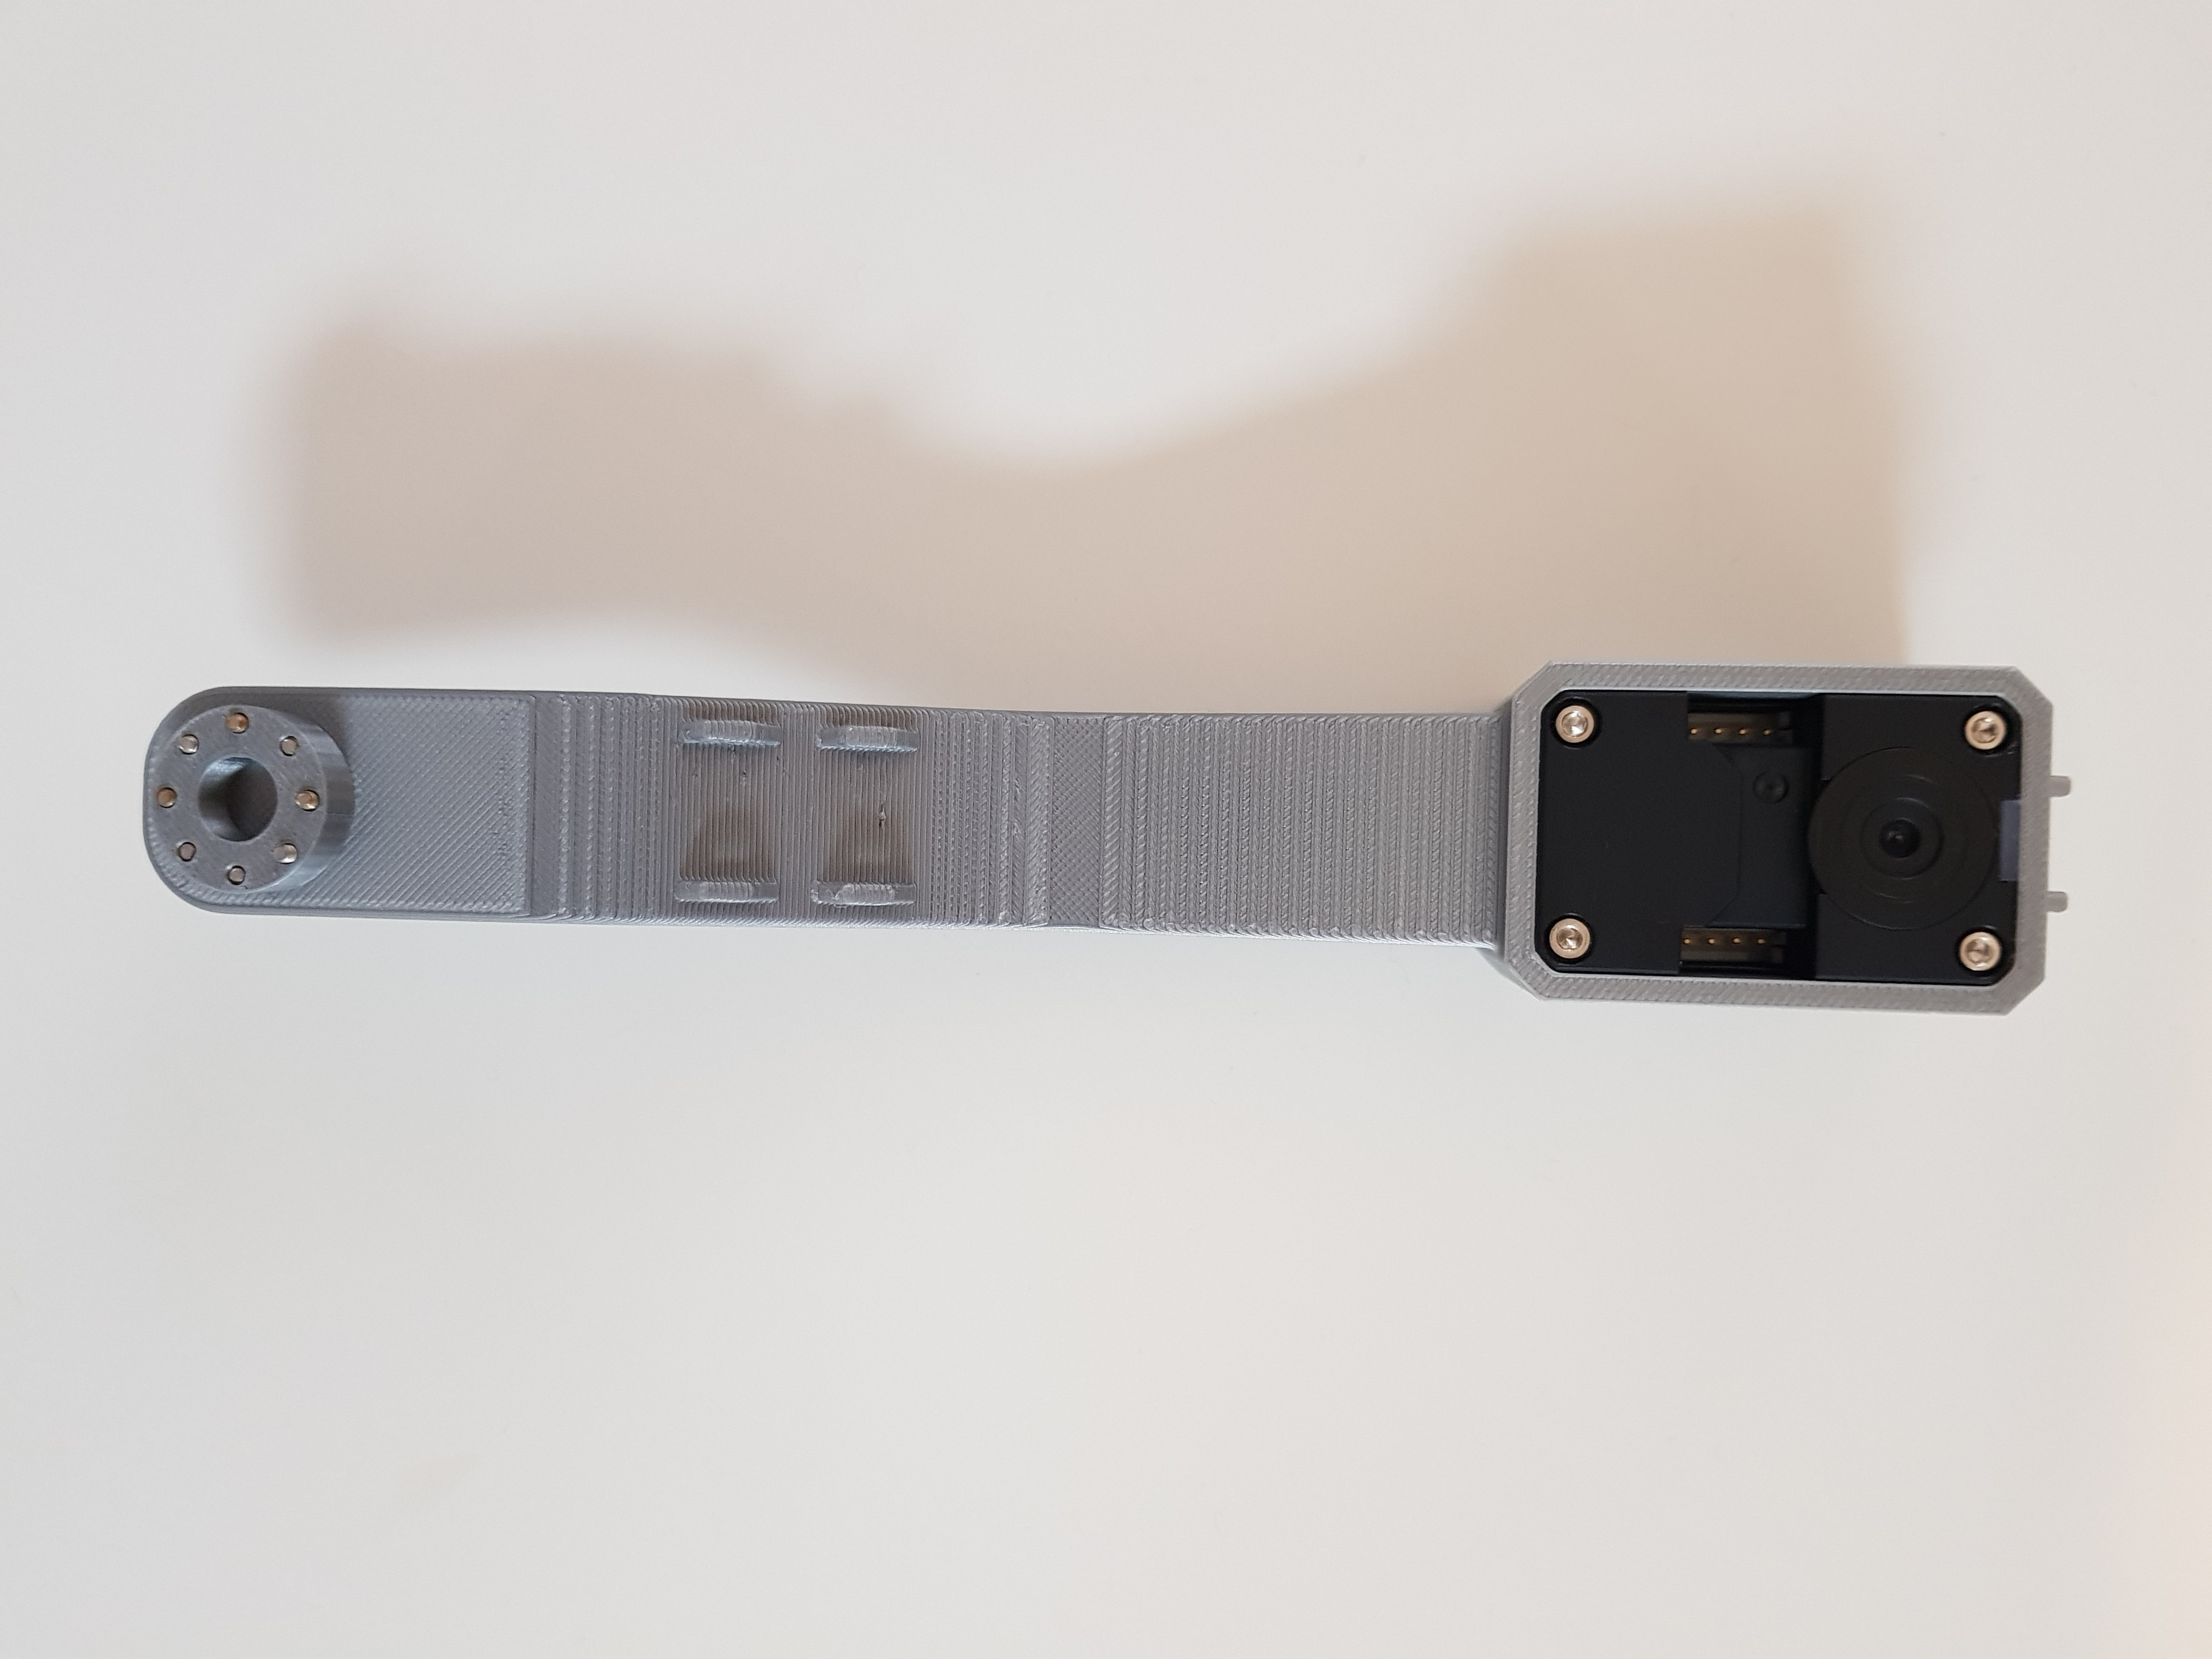
\includegraphics[height=0.7\textwidth]{mounting_motors_on_hip_knee_links_2}
		\caption{Mounting motors on hip knee links top view}
		\label{fig:mountingmotorsonhipkneelinkstopview}
	\end{subfigure}
	\caption{Mounting motors on hip knee links}
	\label{fig:Mounting motors on hip knee links}
\end{figure}
%%figure for mounting the motors on the hip knee links
%\begin{figure}[h]
%	\centering
%	\includegraphics[width=0.5\linewidth]{mounting_motors_on_hip_knee_links}
%	\caption{Mounting motors on hip knee links}
%	\label{fig:mountingmotorsonhipkneelinks}
%\end{figure}
%two subfigures for assembling the knee wheel links and hip knee links
\begin{figure}[h]
	\centering
	\begin{subfigure}[t]{0.45\textwidth}
		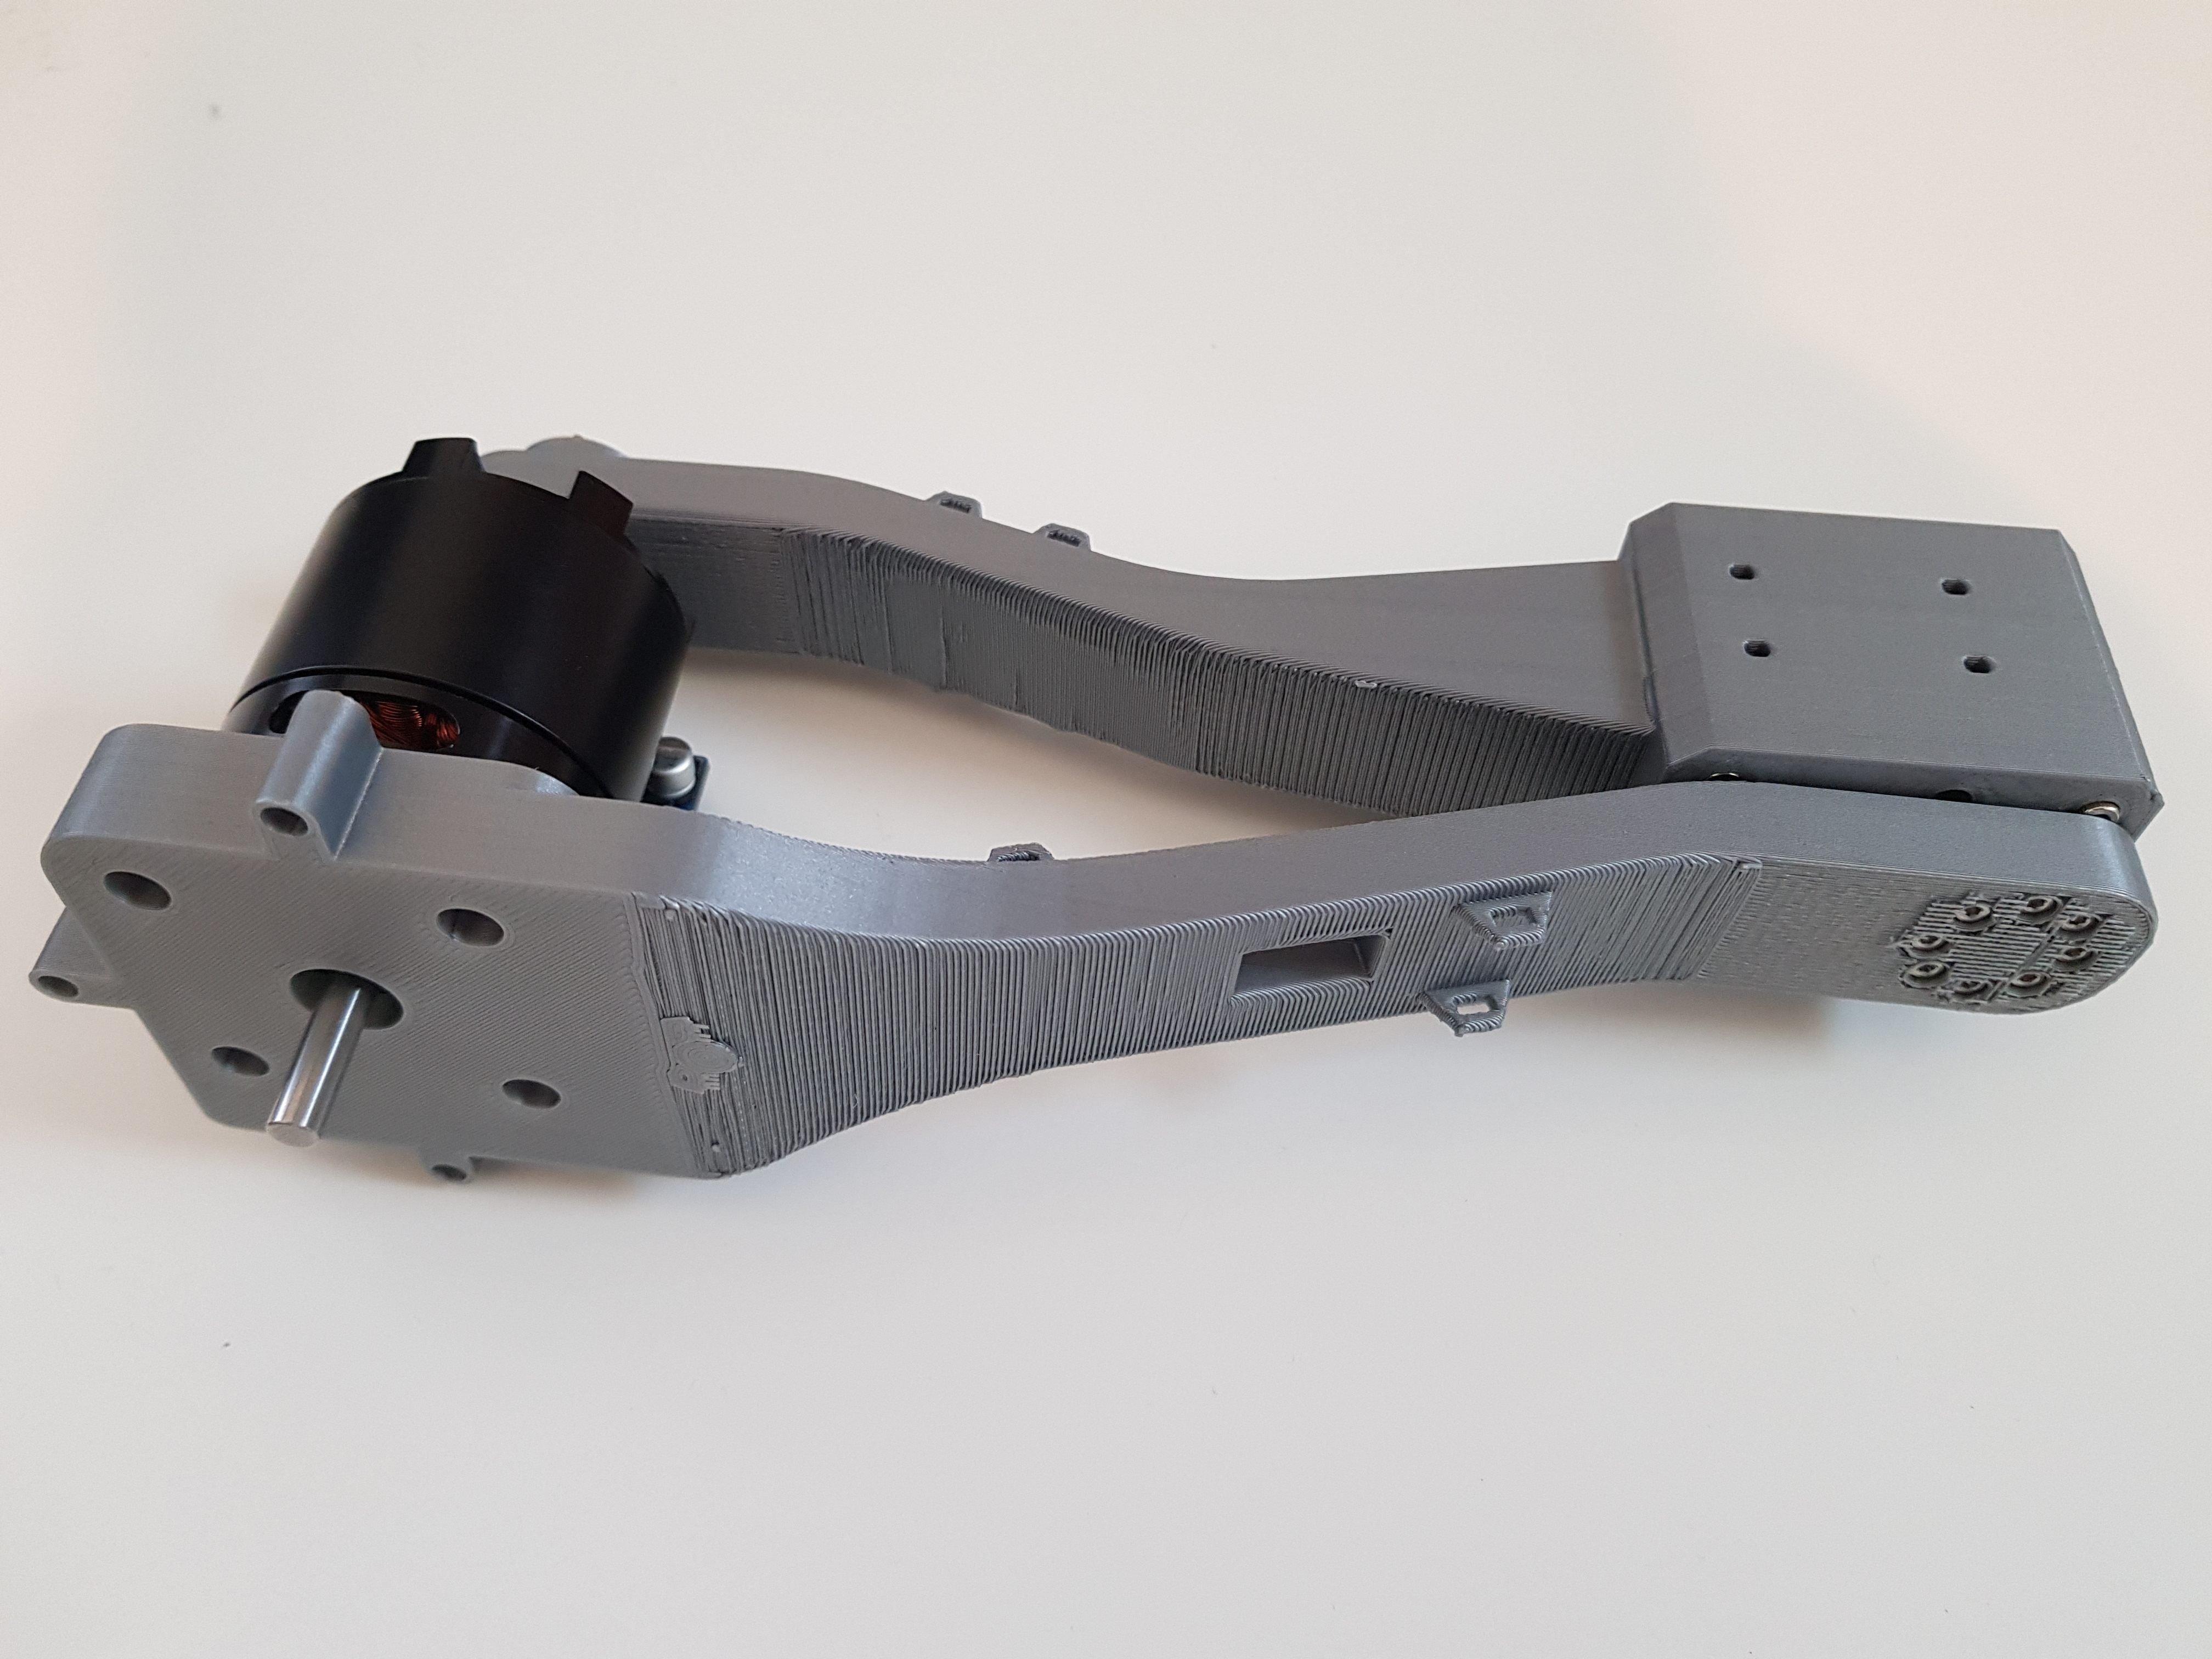
\includegraphics[height=0.7\textwidth]{assembling_knee_wheel_links_and_hip_knee_links_1}
		\caption{Assembling knee wheel links and hip knee links	prespective view}
		\label{fig:assemblingkneewheellinksandhipkneelinksprespectiveview}
	\end{subfigure}
	\begin{subfigure}[t]{0.45\textwidth}
		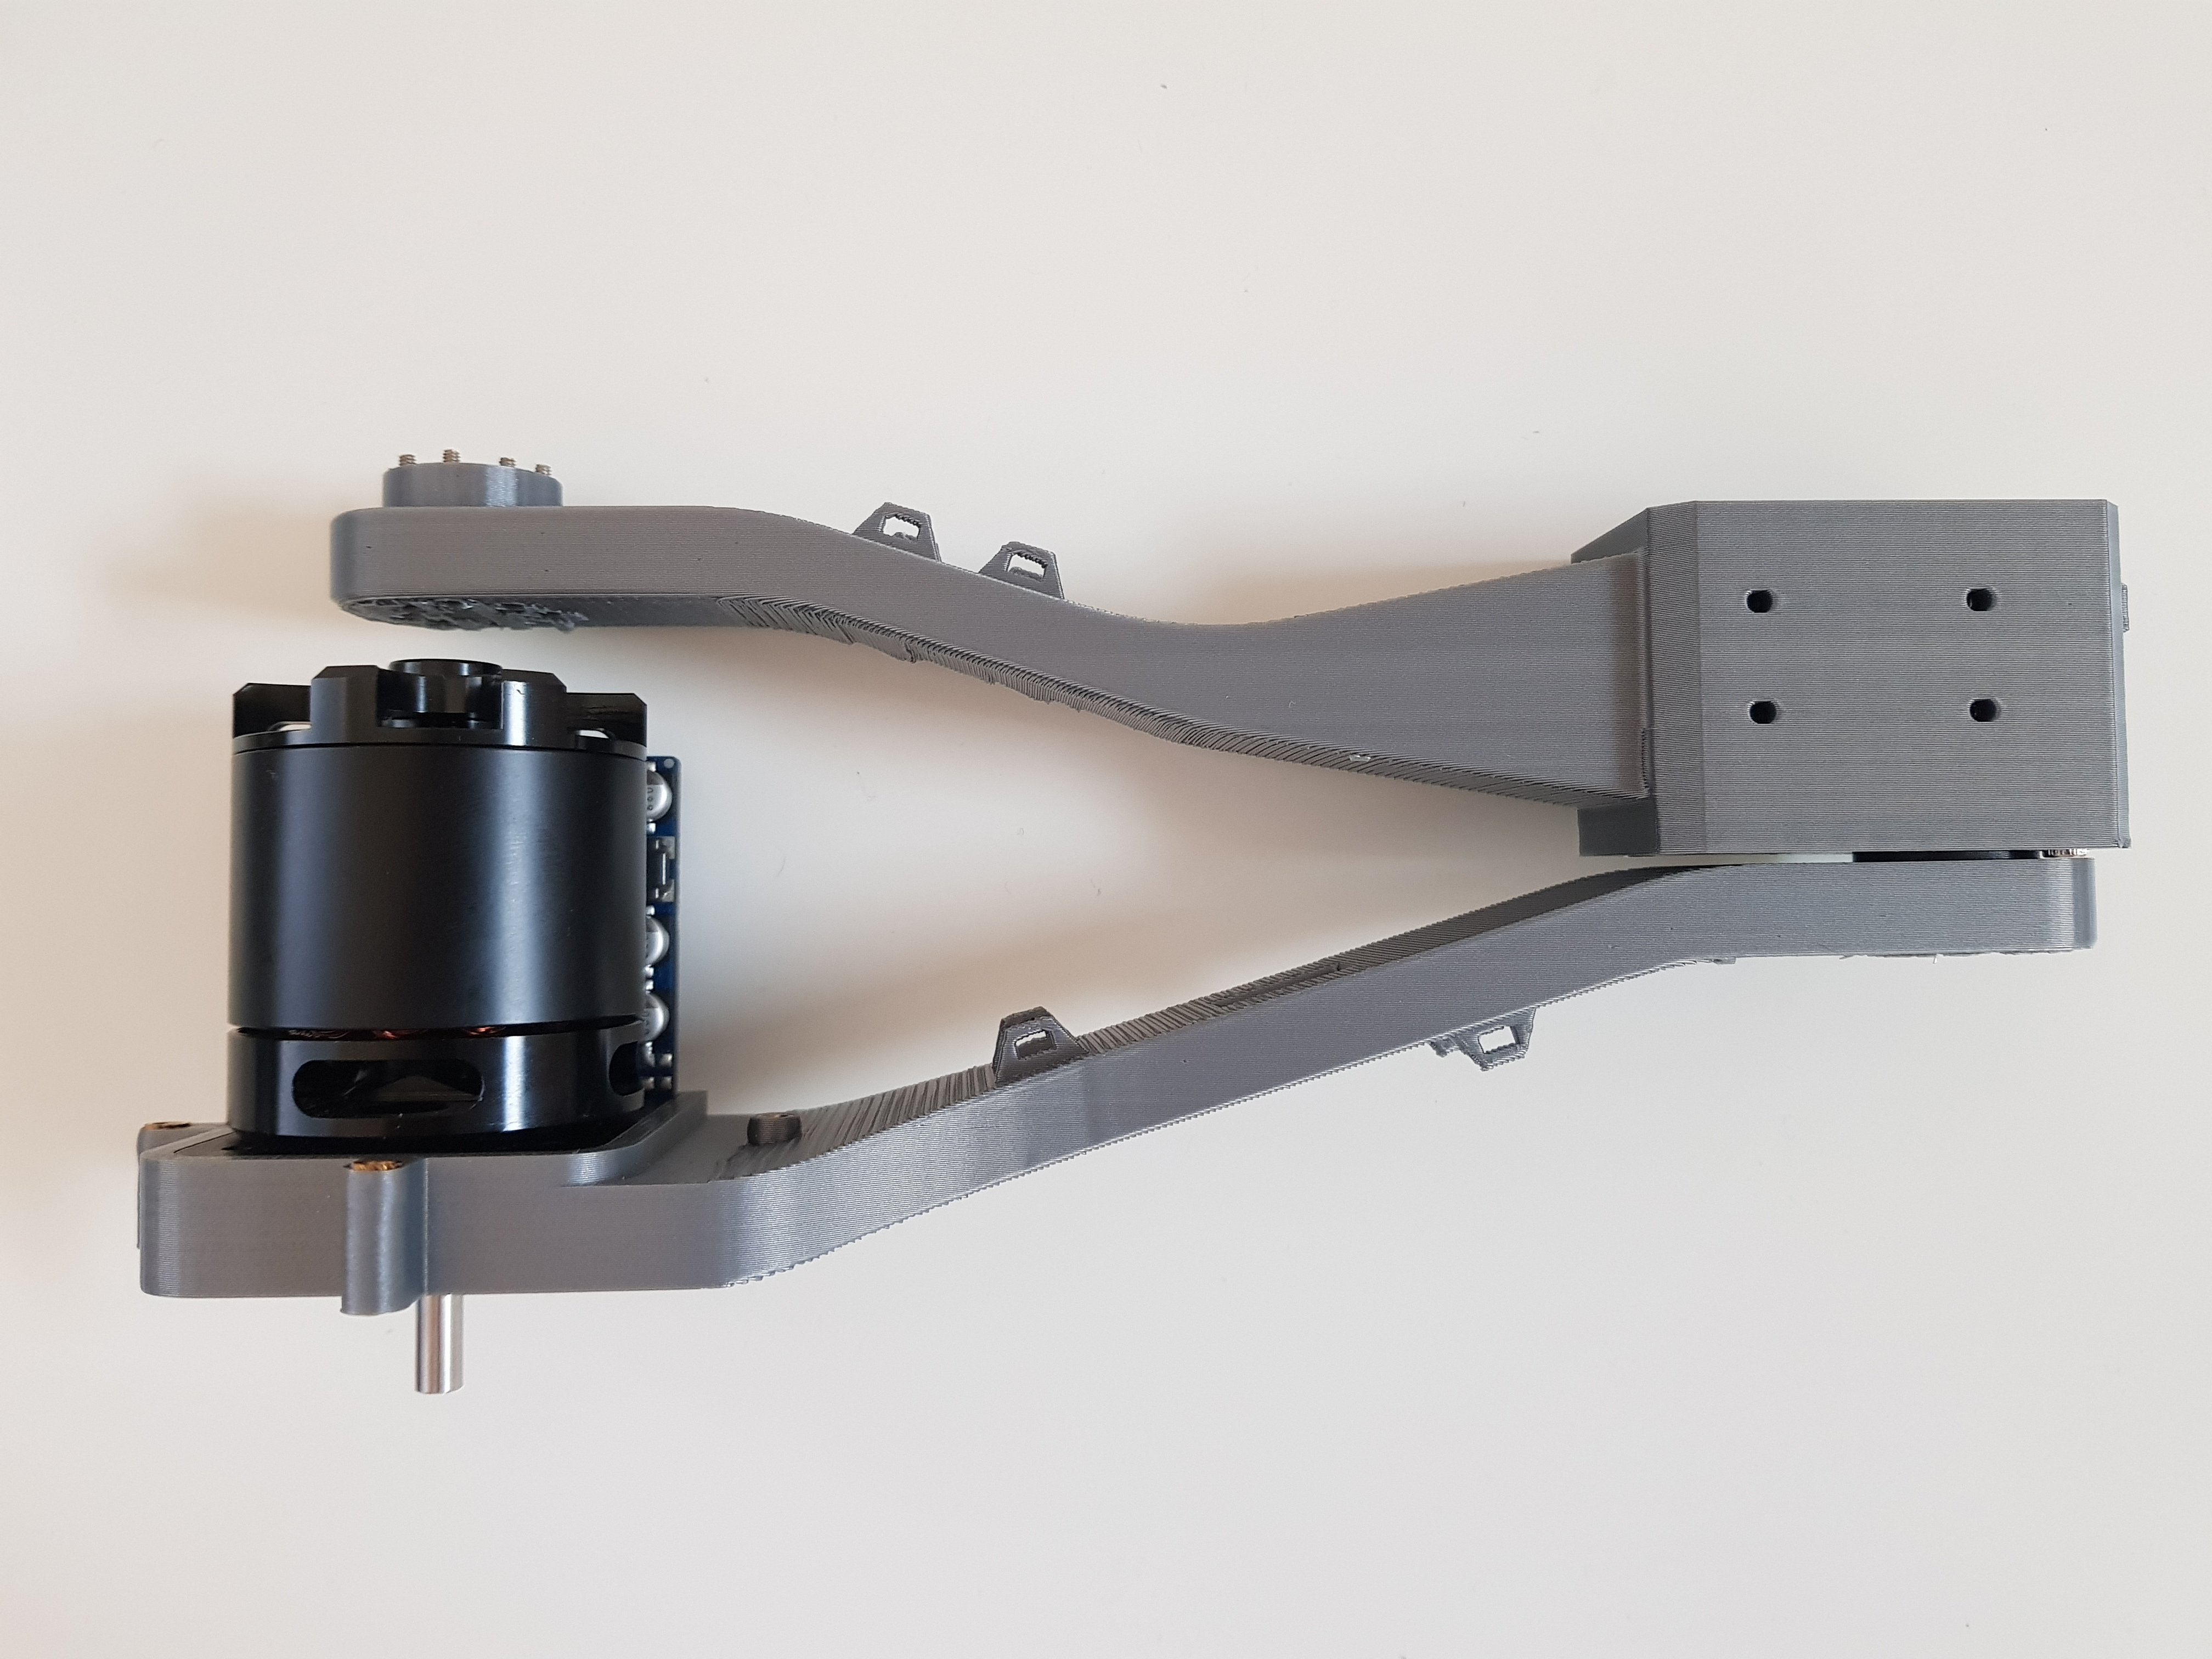
\includegraphics[height=0.7\textwidth]{assembling_knee_wheel_links_and_hip_knee_links_2}
		\caption{Assembling knee wheel links and hip knee links	top view}
		\label{fig:assemblingkneewheellinksandhipkneelinkstopview}
	\end{subfigure}
	\caption{Assembling knee wheel links and hip knee links}
	\label{fig:Assembling knee wheel links and hip knee links}
\end{figure}
The XM430-W350 motors were mounted into the 

%%figure for assembled knee wheel links and hip knee links
%\begin{figure}[h]
%	\centering
%	\includegraphics[width=0.5\linewidth]{assembled_knee_wheel_links_and_hip_knee_links}
%	\caption{Assembled knee wheel links and hip knee links}
%	\label{fig:assembledkneewheellinksandhipkneelinks}
%\end{figure}
%figure for the assembing the body hip knee links.
\newpage
\begin{figure}[h]
	\centering
	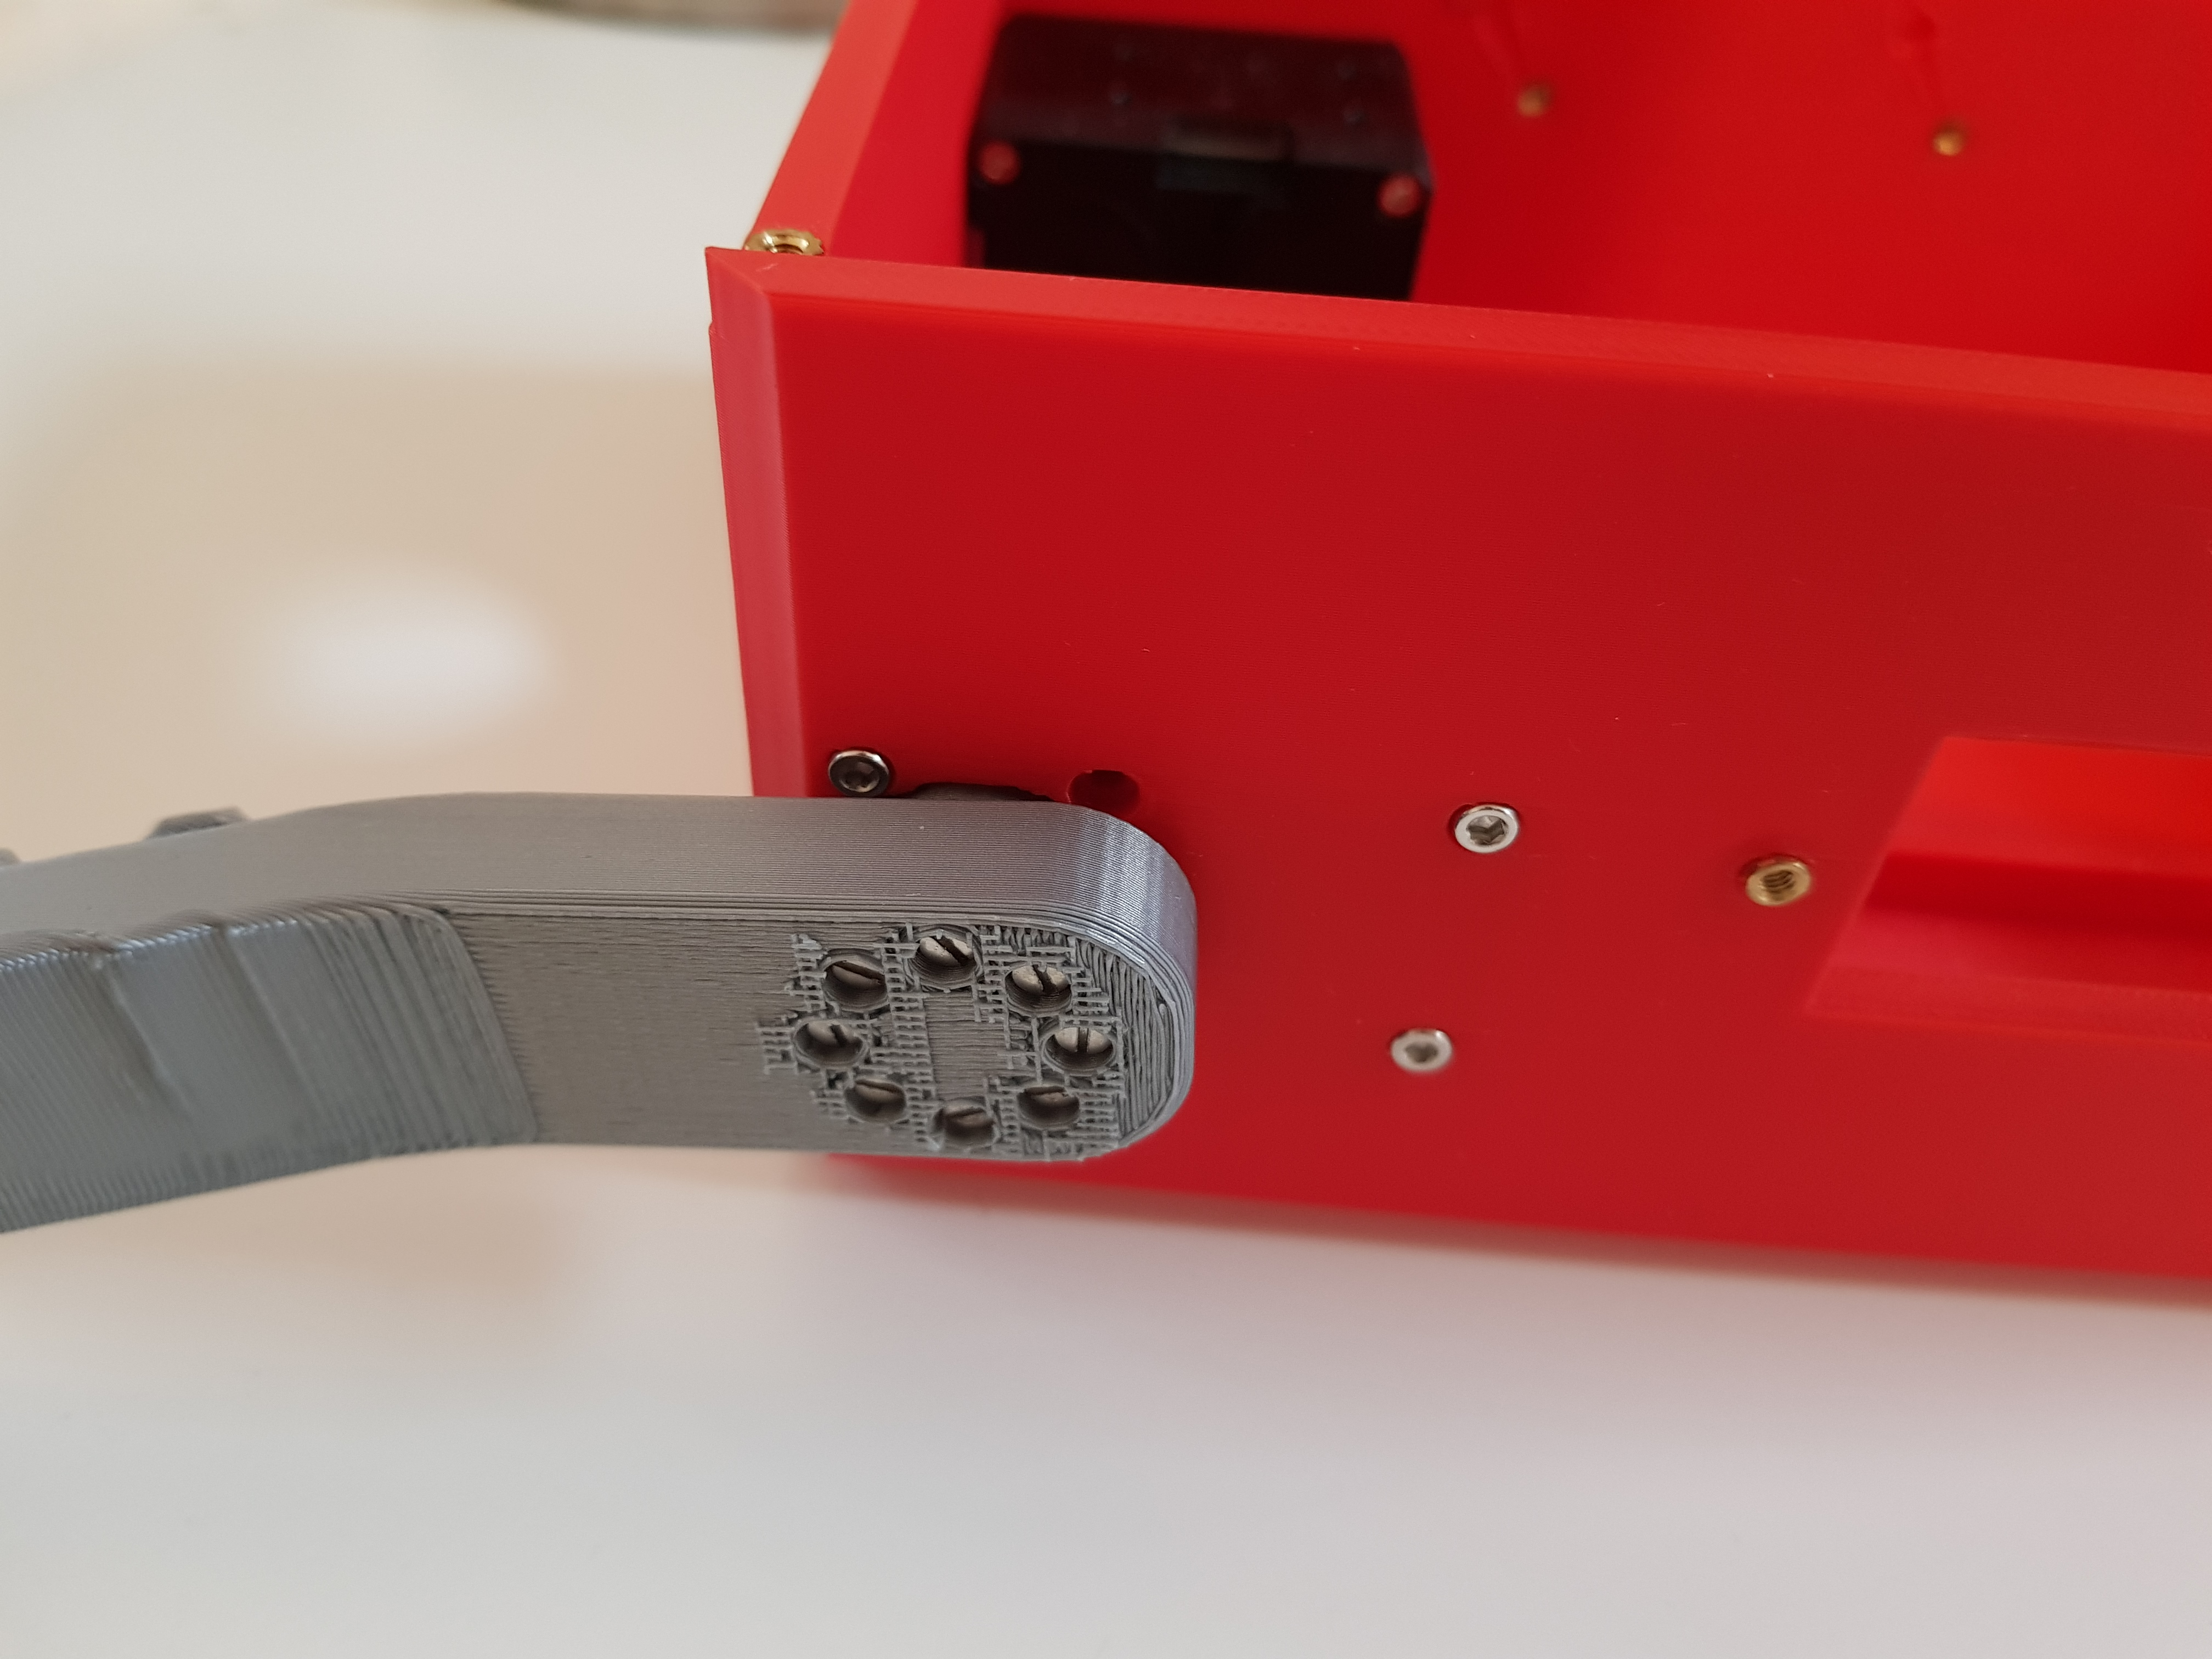
\includegraphics[width=0.5\linewidth]{assembling_body_hip_knee_links}
	\caption{Assembling body to hip knee links}
	\label{fig:assemblingbodyhipkneelinks}
\end{figure}
The hip knee links were assembled to the body using sixteen screws as shown in figure \ref{fig:assemblingbodyhipkneelinks} to the hip motor horns after the motors were mounted in the body.
%figure for fully assembled chassis
\begin{figure}[h]
	\centering
	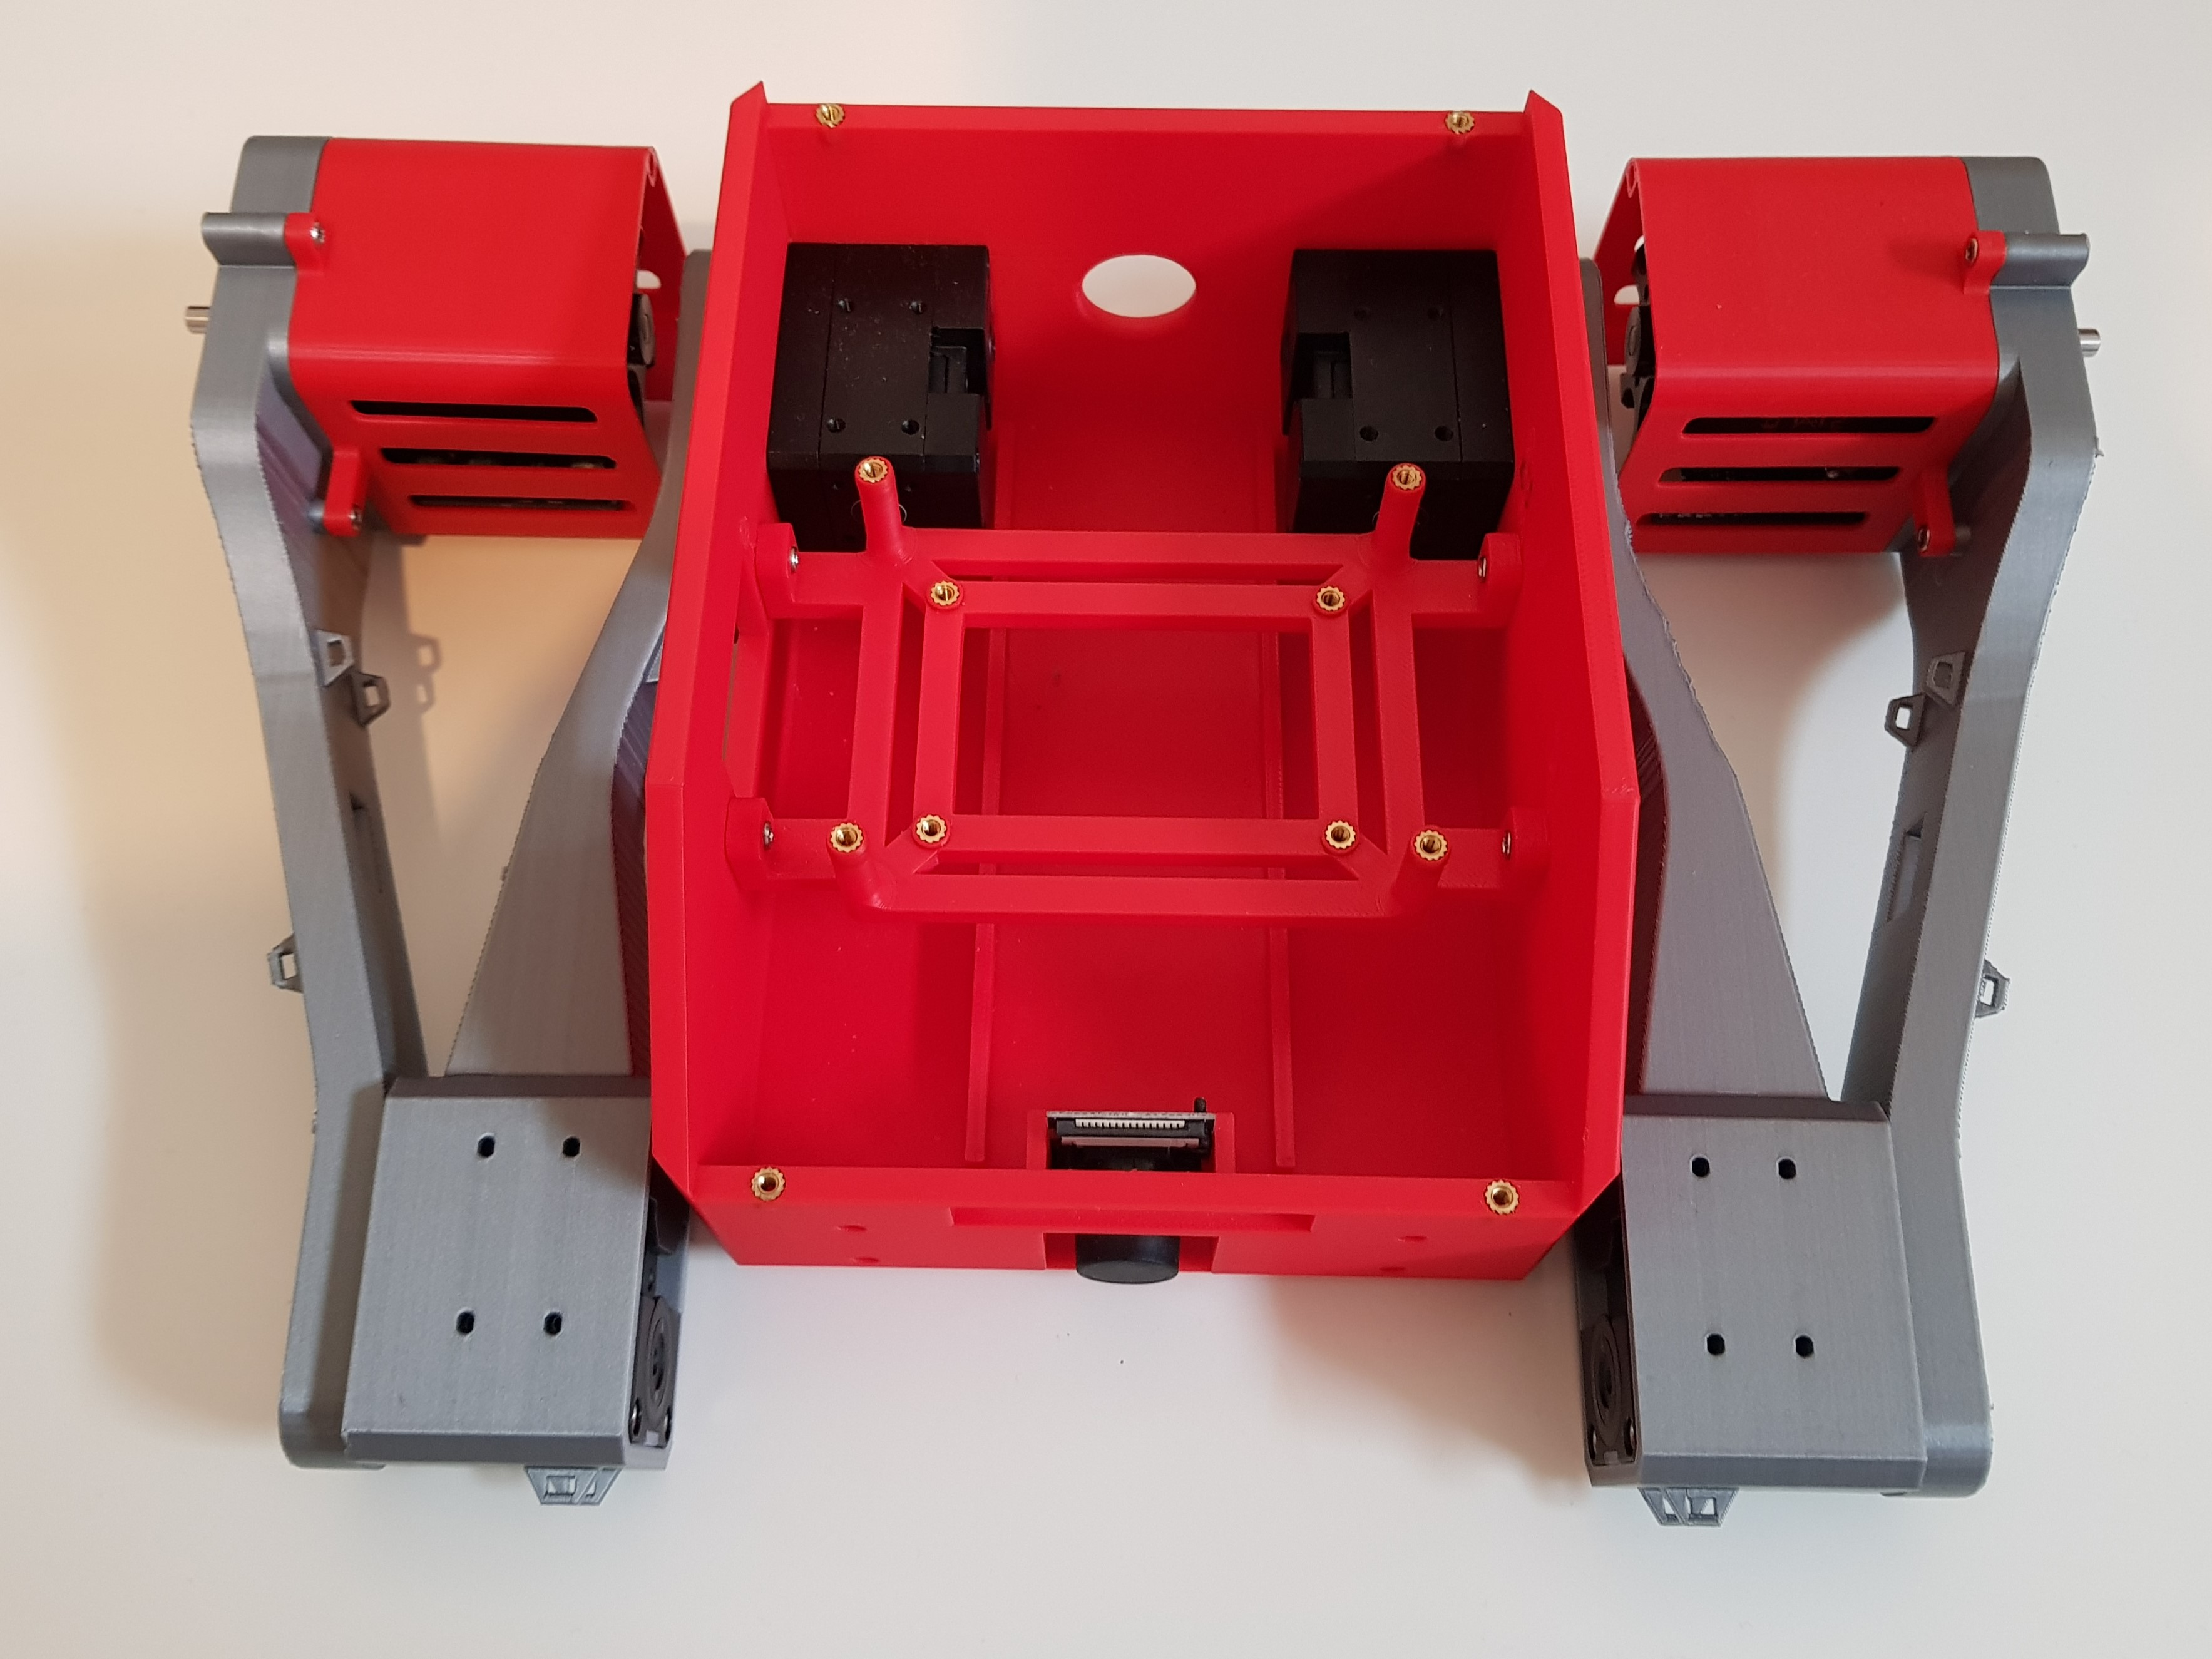
\includegraphics[width=0.5\linewidth]{fully_assembled_chassis}
	\caption{Fully assembled chassis}
	\label{fig:fullyassembledchassis}
\end{figure}

\section{Integration of Mechanical and Electronic Systems}

%how the electronics were mounted on the chassis

\subsection{Wiring tree}
%how the wiring was made
According to the wiring tree in the electrical design chapter, the wiring tree was made to fit the lengthes between the components.
%figure for the wiring tree
%\begin{figure}[h]
%%	\centering
%%	\includegraphics[width=0.5\linewidth]{wiring_tree}
%%	\caption{Wiring tree}
%%	\label{fig:wiringtree}
%%\end{figure}
%

\subsection{Electronics Assembly}
%figure for the electronics mounted on the board mounting rack
\begin{figure}[h]
	\centering
	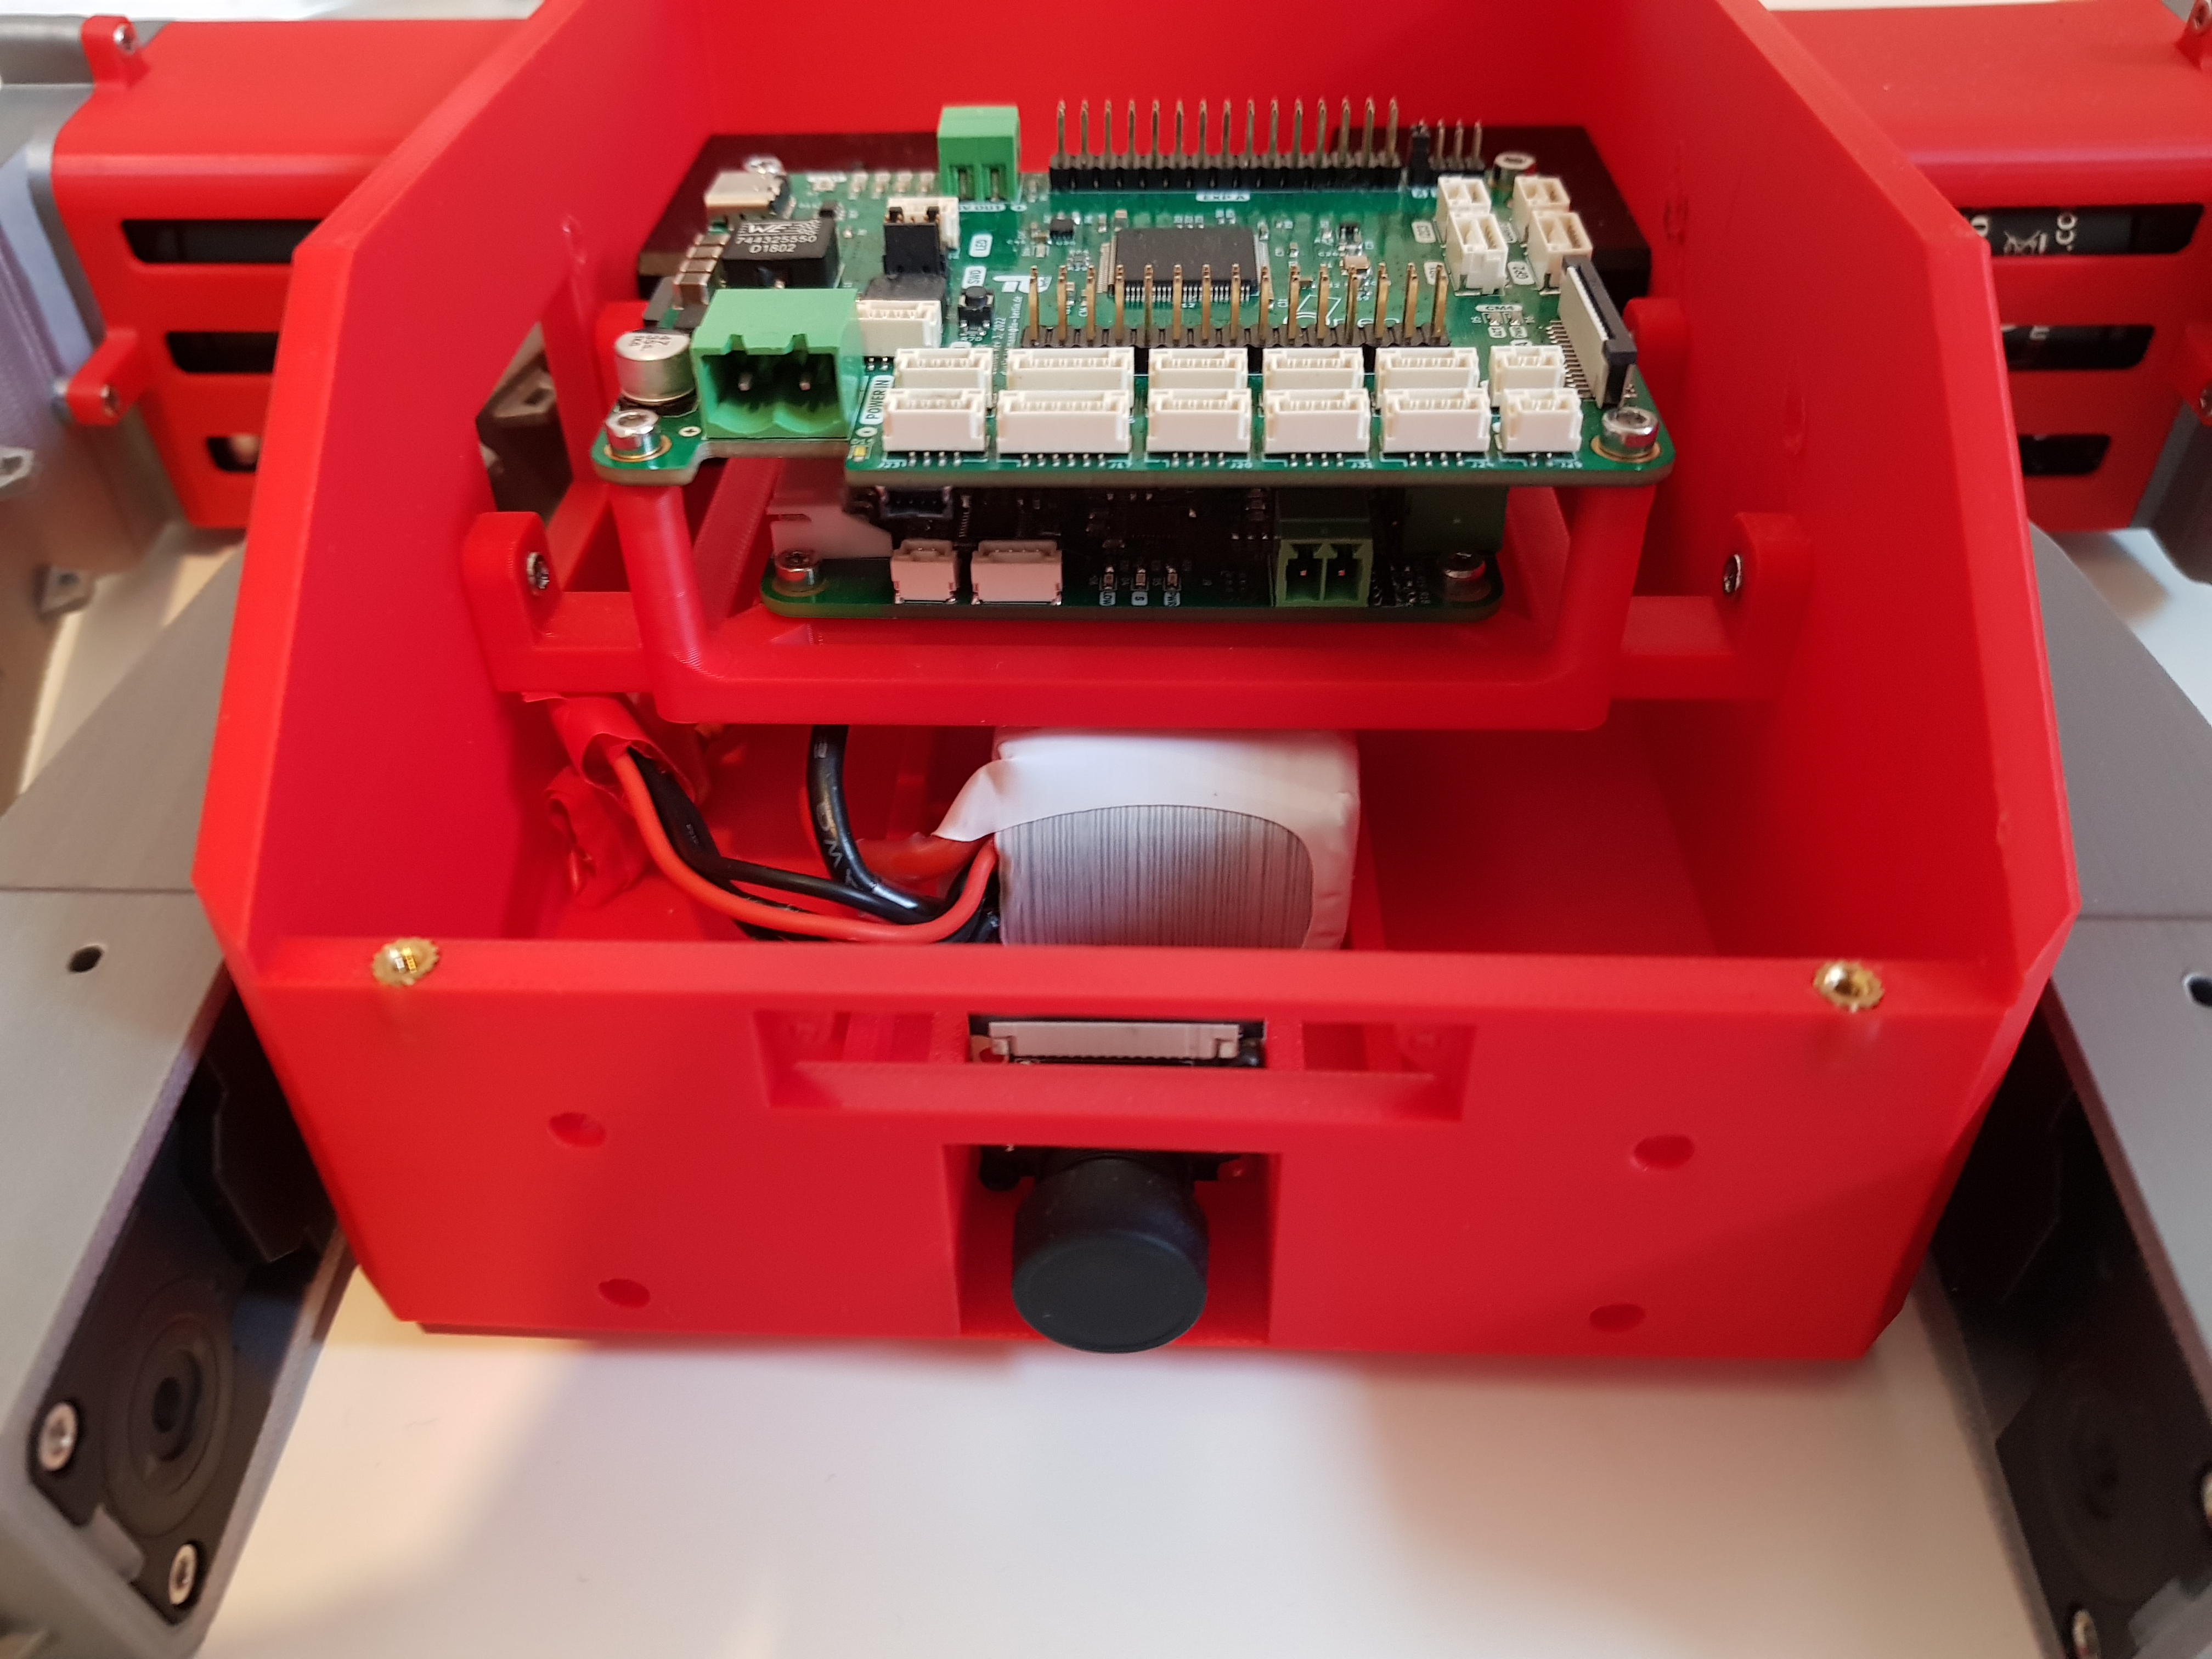
\includegraphics[width=0.5\linewidth]{electronics_mounted_on_board_mounting_rack}
	\caption{Electronics mounted on board mounting rack}
	\label{fig:electronicsmountedonboardmountingrack}
\end{figure}
%the process of connecting the wires to the board.
%measurments of the wires used
\begin{itemize}
\item Discussion on how mechanical components interface with electronic systems.
\item Challenges faced in integration and strategies employed to overcome them.
\end{itemize}

\section{Troubleshooting and Problem Solving}
%the knee motor was touching the screw so we had to shorten the screw
%the knee motor didn't fit in the link two solutions were considered either to file the link or to reprint with new dimentions.
\begin{itemize}
\item Discussion of any unexpected challenges or issues faced during assembly.
\item How these issues were diagnosed and resolved.
\end{itemize}
\section{Safety Considerations}
%cable lengthens
% cables touching the motors
\begin{itemize}
	\item Safety measures taken during the assembly process.
	\item Design considerations for ensuring the operational safety of the robot.
\end{itemize}
\begin{itemize}
	\item \textbf{Discrete Numerical Simulation:} Elaboration on the process of discrete numerical simulation, including the discrete double integration method to arrive at the state vector.
\end{itemize}

\begin{notebox}
	the bolts used the problem to shorten them so that it wouldn't touch the motor 
\end{notebox}

